% Copyright (c) 2014,2016 Casper Ti. Vector
% Public domain.

\chapter{实验评估} \label{chap:evaluation}

\section{实验方法}

我们的实验测试机器采用了英特尔至强Xeon E5-2699 v4处理器。该处理器支持CAT技术,拥有22个处理器核心,它们共享一个20路、大小为55MB的L3缓存,每一个缓存路的容量为2816KB。处理器一共包含16个CLOS,也就是说最多支持16种不同的分配。此外,每个核有一个32KB的私有L1指令缓存、一个32KB的私有L1数据缓存和一个256KB的私有L2缓存。因为多级采用了包含式设计,所以在CAPS中我们并没有考虑私有的L1和L2缓存。该实验环境的内存带宽为76.8GB/s,同时拥有64GB的内存,所以内存竞争的干扰因素较小。我们把测试程序封装到Docker中,每个Docker中运行一个不同的测试程序,并把各个Docker绑在不同的核上。我们通过一个英特尔提供的开源工具来执行CAT分配~\parencite{pqos}。因为不同的程序执行的时间长短也不一样,运行结束的时间点也会不同,在测试时,我们会让早结束的程序反复执行,直到最慢的程序执行完毕。在程序实时运行的同时,一些关键参数,比如运行时IPC、LLC失效数等等会通过硬件计数器(Performance Counter)统计收集,并且真实的缓存大小占用也通过会缓存监控技术(CMT)进行采集。

我们从SPEC CPU2006中选择了20个测试程序作为我们的评估对象,如表\ref{tab:benchmarks}所列。从中我们选择4到15个不同的程序组成一个并发执行的工作负载。虽然我们也想尝试测试更大的并发度,但是由于目前最高端的处理器只支持16个CLOS,同时一个默认的CLOS需要留给操作系统等其他程序,所以目前最大支持的并发度就是15。

对于每个程序,我们采用第\ref{sec:prediction_sample}节介绍的方法进行离线采样分析,得到每个程序的失效率曲线和访存频率,这两个特征会被预测模型所用到。为了了解多程序工作负载中各个程序的的特性,我们进一步将这20个测试程序分成了三个类别,如表\ref{tab:benchmarks}所示。这种分类方式和前人所提倡的类似~\parencite{lin2008gaining}。分类依据两个维度来考察每个程序:敏感度和污染度。敏感程度代表程序从缓存中的收益,一个敏感型程序会从较大的缓存占用获得较大收益,反之如果缓存占用较小会收到较大损害;而一个缓存不敏感的程序无论分配的缓存是大是小都不会受到太大影响。这里我们用缓存分配从6MB下降到1MB引起的程序运行效率的下降(Slowdown)来量化程序的敏感程度。由于CAT分配下一个路的大小动辄就几MB,所以Slowdown无法通过实测来得到。这里我们通过失效率曲线来估计程序的Slowdown。污染度主要指的是在竞争中该程序所能抢占的缓存多少,抢占的越多,别的程序得到的就越小,说明污染程度越重。污染度主要跟程序的访存频率相关,一般访存指令越多污染程度就越高。通常情况下,缓存敏感的程序因为有大量的访存指令,所以会占据较多缓存。但反过来并不成立,污染度较高的程序并不一定都是缓存敏感的。

我们把Slowdown大于10\%的归位A类。这一类程序对缓存敏感,同时它们通常也有较大的缓存需求,在竞争中会占用较多缓存资源,A类测试程序一共有9个,剩下11个程序根据它们的访存指令占比进一步划分为B类和C类。Slowdown小于等于10\%且每1000条指令的L3访存数大于5的程序被归位B类,这一类程序是不敏感但污染度较高的程序。B类程序有5个,它们会侵占大量的缓存然而并不会从中受益很多。最后,剩下的6个程序被归位C类,它们的Slowdown小于10\%,并且每1000条指令造成的L3访问也小于5,这一类程序属于既不敏感也不污染。多程序工作负载中A类、B类和C类程序的比例可能会对优化效果有影响,为了模拟各种情形,我们在实验中采用了不同的配比。

\begin{table}[htbp]
\caption{Benchmark classification}
\label{tab:benchmarks}
\centering
\begin{tabularx} {1\textwidth}{|l|l|l|X| } 
 \hline
 Type & Slowdown & APKI & Benchmarks \\
 \hline
 A & $> 10\%$ & $> 5$ & 401.bzip2 403.gcc 429.mcf 436.cactus 465.tonto 470.lbm 471.omnetpp 473.astar 482.sphinx\\ 
 \hline
 B & $\leq 10\%$ & $> 5$ & 410.bwaves 434.zeusmp 437.leslie3d 459.GemsFDTD 462.libquantum\\ 
 \hline
 C & $\leq 10\%$ & $\leq 5$ & 433.milc 445.gobmk 453.povray 456.hmmer 458.sjeng 464.h264ref\\
 \hline 
\end{tabularx}
\end{table}

正如在第\ref{sec:opt_goals}节所介绍的,我们选择并实现了5种优化策略,分别针对5种指标:平均失效数(Average MPKI)、吞吐量(Throughput)、平均效率下降(Average slowdown)、公平效率下降(Fair slowdown)和最大效率下降(Maximum slowdown)。前3个主要针对系统的综合性能,Fair slowdown兼顾了公平性和性能,而Maximum slowdown表示了QoS和性能。因为除了CAPS以外,目前并没有一个可以在真机上运行的优化框架可以做比较,所以我们实验只和完全竞争,以及无重叠分配方案做了比较。完全竞争就是传统意义上自由共享的LLC,也可以被认为所有分配都包含整个LLC且完全重叠。不重叠方案是前人研究普遍采用的分配方式,各个分配之间无重叠无共享。我们通过检索所有可能的无重叠方案,分别输入到CAPS预测模型中进行预测,然后找到一个最优的无重叠方案。因为重叠不存在,所以CAPS预测模型无需迭代,只要经过一次计算就可以得到预测结果。

我们对75个不同的工作负载进行实验,负载中包含的测试程序数从4个到15个不等。在下一节的实验结果中,我们在这5种优化目标下,分别对比了CAPS部分重叠方案、无重叠方案和完全重叠的自由竞争。

\section{实验结果}

因为预测模型是优化算法的基础,它的准确率对优化效果有重要影响。在我们的所有实验中,CAPS预测模型对失效率预测的平均准确率高达90.5\%,对IPC的预测平均准确率高达80.1\%,单次的预测时间平均为0.01秒。所以该预测模型无论从准确率还是开销上,都可以被接受。

\begin{figure}[htbp]
\centering
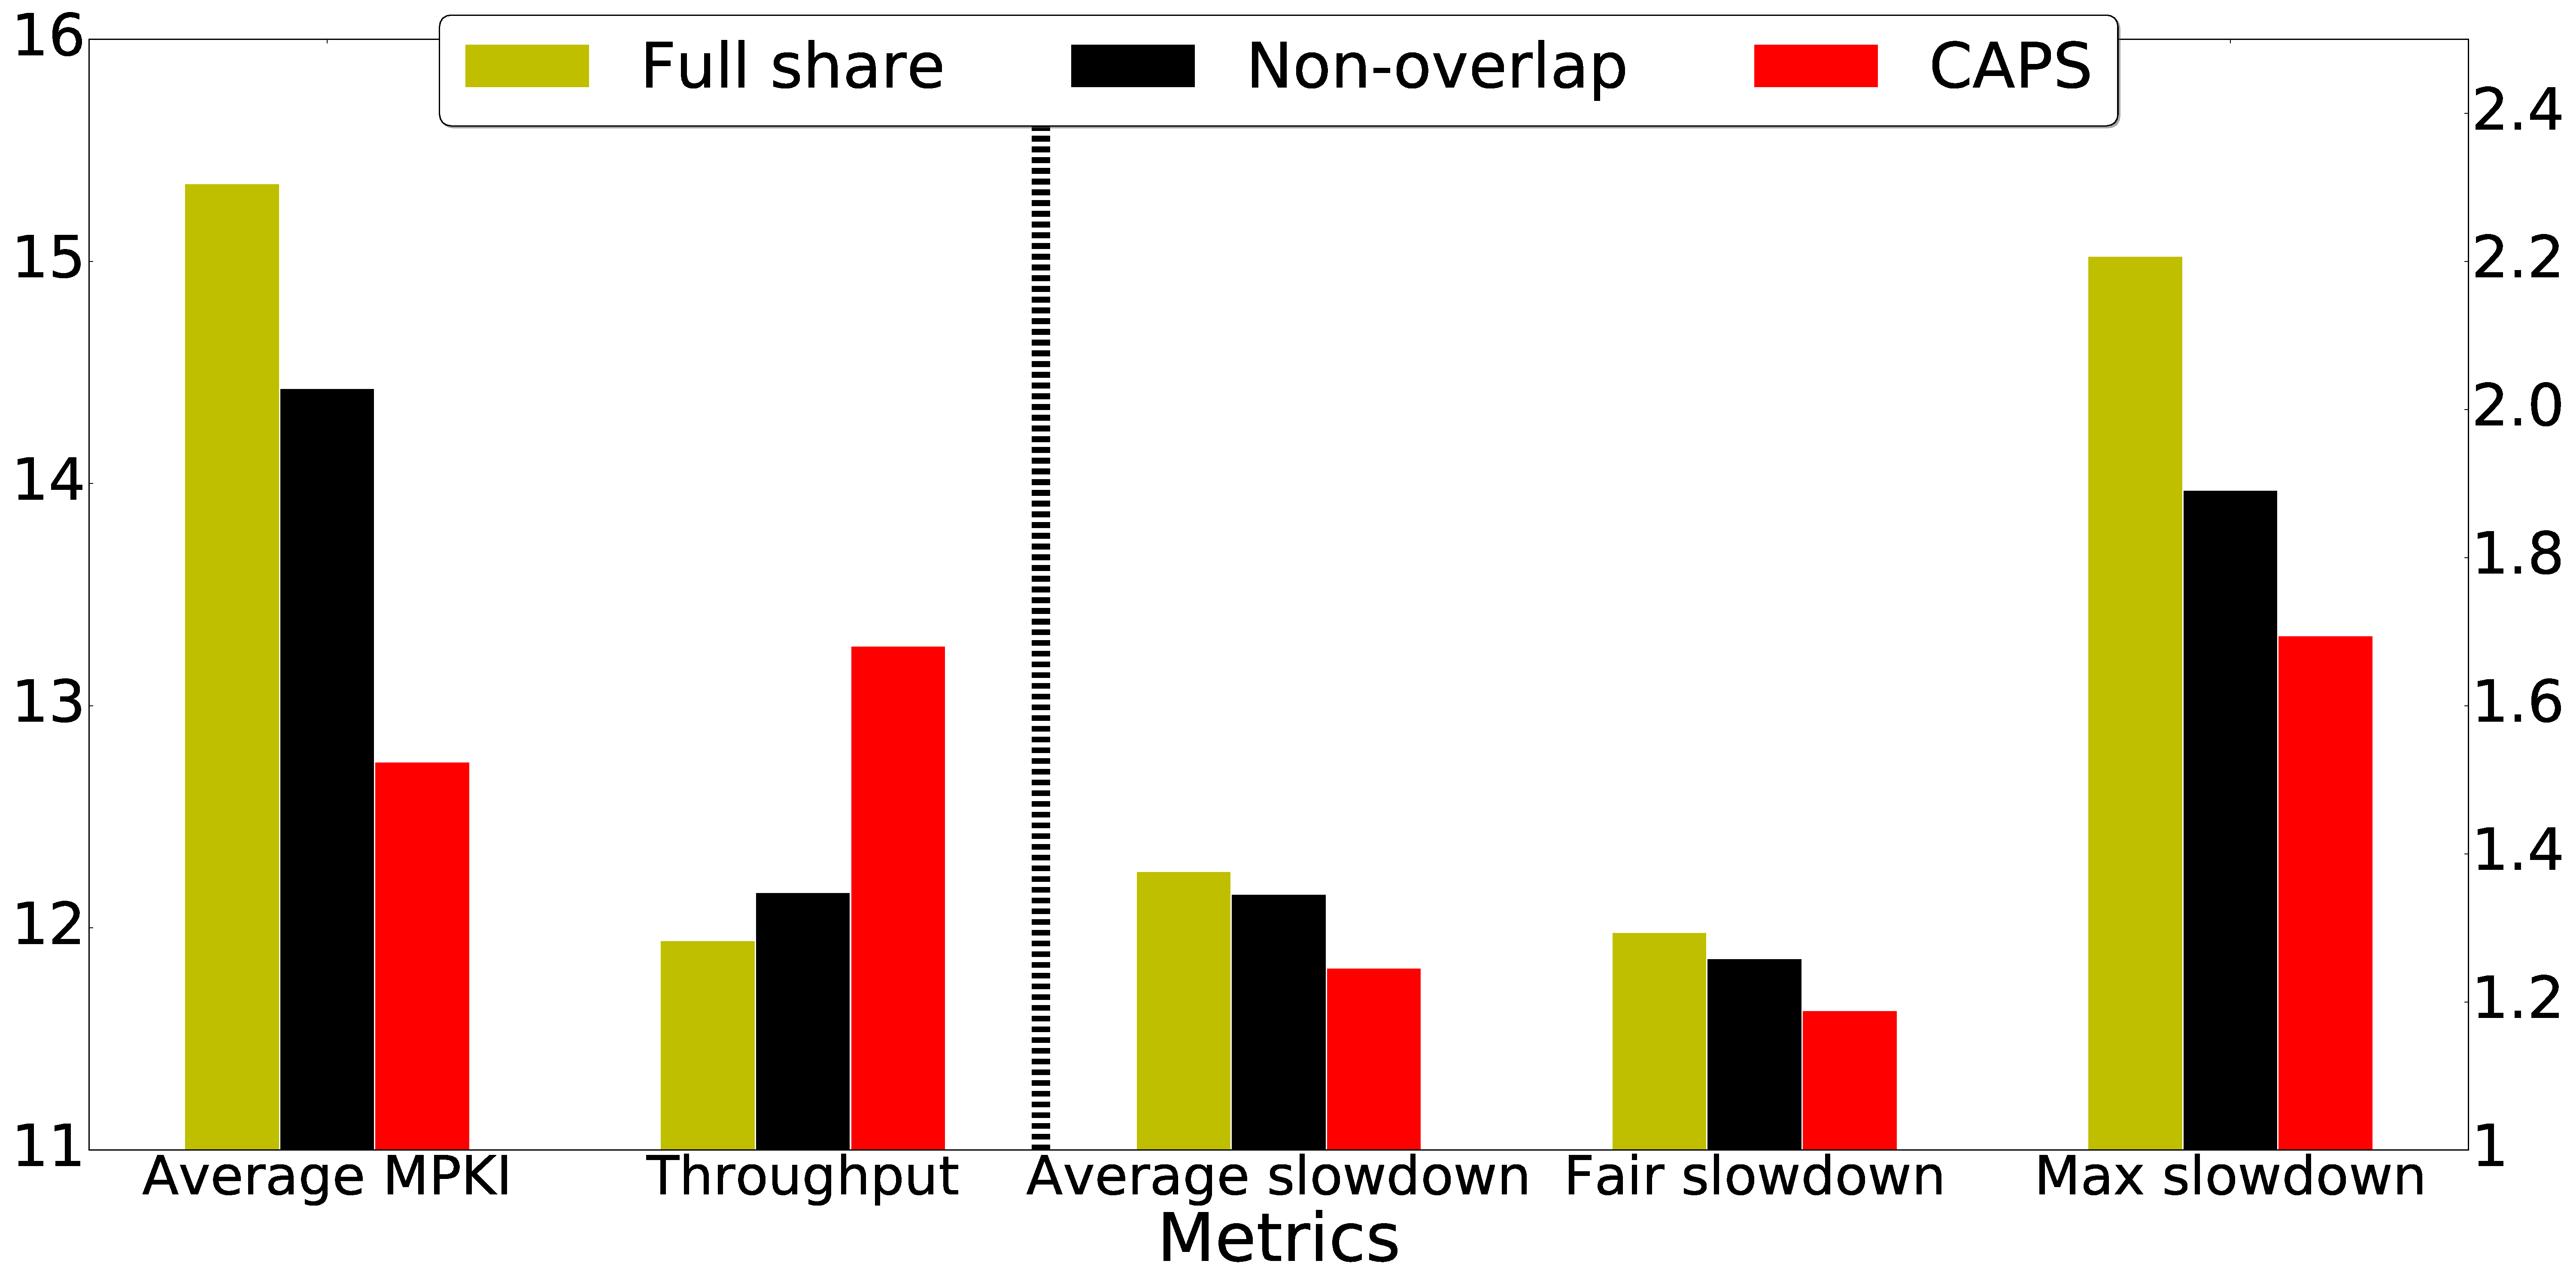
\includegraphics[width=0.9\columnwidth]{figures/avg_analysis.pdf}
\caption{完全重叠、不重叠与CAPS部分重叠方案的平均性能对比}
\label{fig:avg_an}
\end{figure} 

我们实现了5种优化目标。Average MPKI、Average slowdown、Fair slowdown和Maximum slowdown是越小越好的指标,而Throughput是越大越好的指标。对于每一个指标,CAPS会输出一个部分重叠的优化分配方案。我们将这个方案在真机上运行,将硬件计数器测量到的参数计算成指标值,与不重叠方案、完全重叠方案进行比较。我们一共测试了75种工作负载:4、6、8、12和15个并发程序的各10种,10个程序的25种。测试的平均结果如图\ref{fig:avg_an}所示。

\begin{itemize}
    \item 对于Average MPKI, CAPS相比于完全竞争在平均情况下可以减少16.96\%的失效数,最好情况下可以减少高达23.1\%。
    \item 对于Throughput,CAPS相比于完全竞争可以平均提升11.11\%,最好情况下可以提升31.3\%。
    \item 对于Average slowdown,CAPS平均可以缓解8.16\%,最好情况下达11.18\%。
    \item 对于Fair slowdown,CAPS平均可以优化8.17\%,最好情况下13.2\%。
    \item 对于Maximum slowdown,CAPS平均可以优化23.24\%,最好情况下33.42\%。
\end{itemize}

通常情况下,在核数/线程数较多时,在缓存敏感和污染程序较多时,CAPS可以提供更好的优化效果。在一共375次比较中(75个工作负载 * 5个指标),CAPS在354中胜出,比完全共享和不重叠方案中最好的那个还要好。CAPS的平均需要20秒左右来生成一个优化方案,这个时间并不包括对程序进行离线采样分析的过程。虽然对于一个离线优化方案,时间开销并不重要,但我们希望在未来可以把CAPS应用的在线实时优化上。对于在线优化的需求,我们可以通过降低算法\ref{alg:opt}的初始温度以及提升降温速度来进一步提升算法那效率。


\section{不同核数的评估分析}

在图\ref{fig:core_count}中,我们比较了在不同核数/线程数的情况下CAPS的优化效果与完全竞争和不重叠分配方案的对比。我们对比了4核、6核、8核、10核、12核以及15核的情况,对于$N$核的情况,我们选取$N$个不同的测试程序,绑在不同的核上同时执行,这样组成一个$N$核的工作负载。对于每一个核数,我们选取10到25种不同的工作负载,这些负载涵盖了不同的A类程序、B类程序和C类程序比例。平均测试结果见图\ref{fig:core_count}。

\begin{figure}[htbp] 
    \centering
    \begin{subfigure}[b]{0.5\linewidth}
        \centering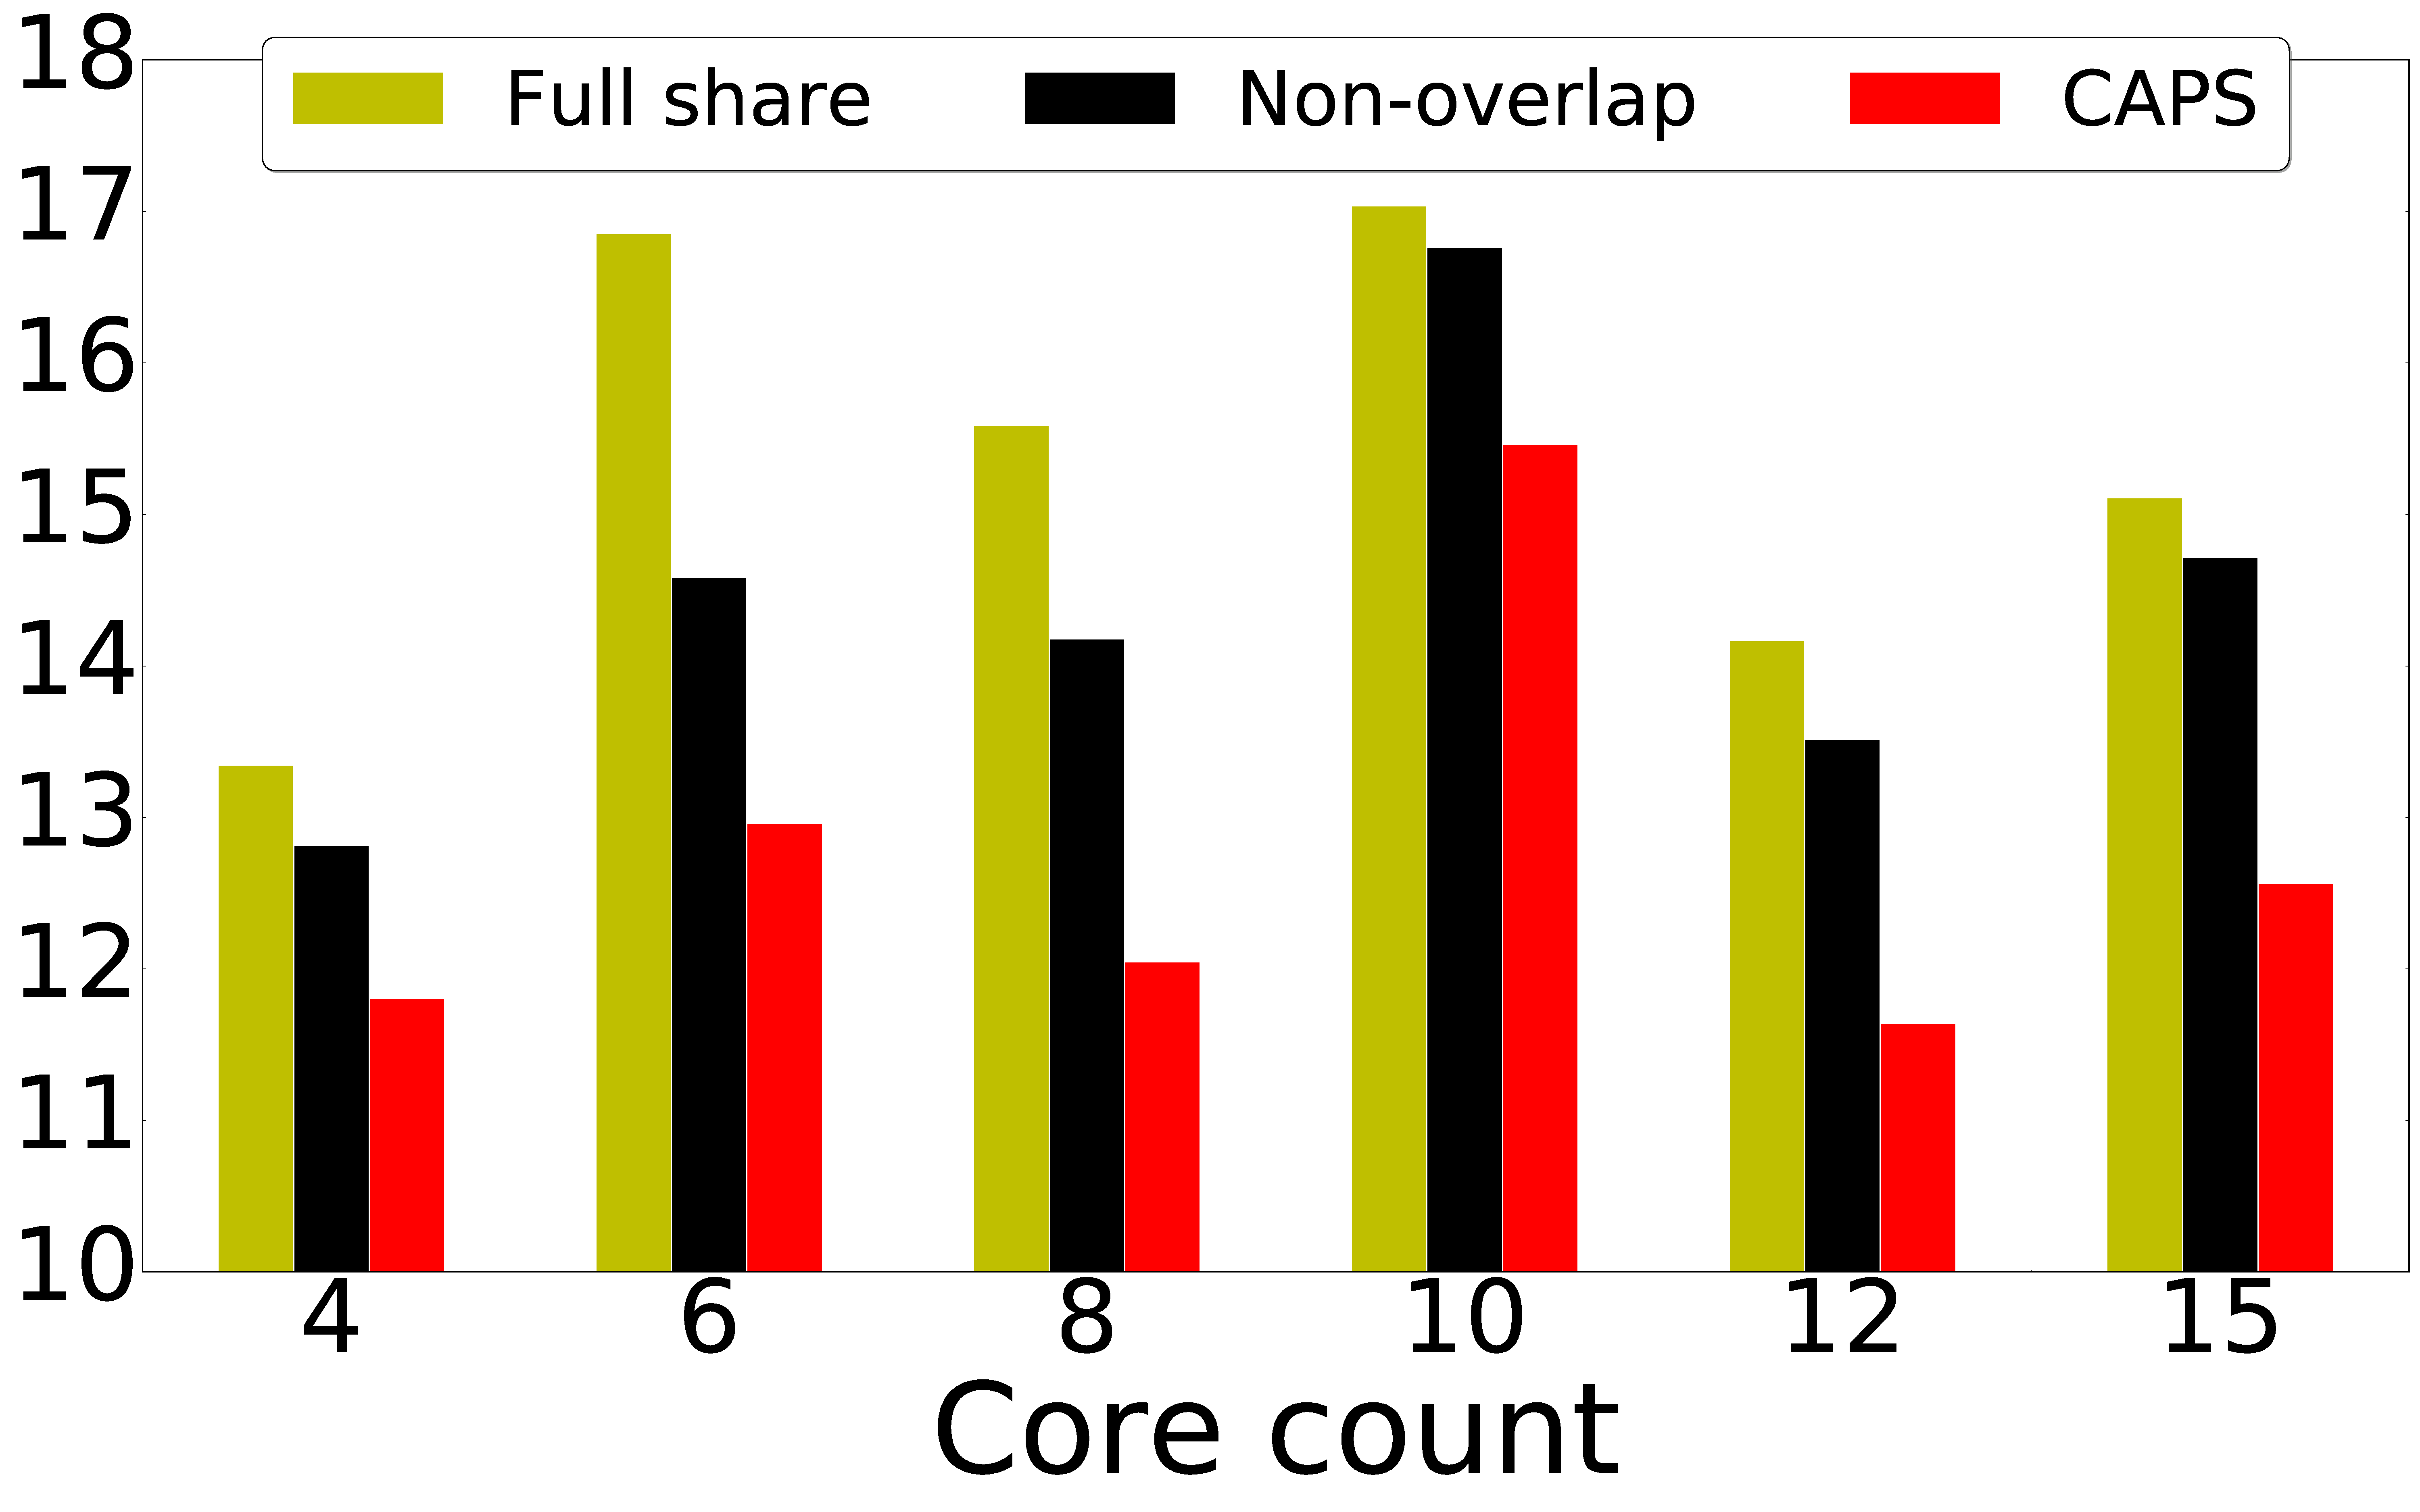
\includegraphics[width=0.9\linewidth]{figures/mpki.pdf}
        \caption{Average MPKI}
    \end{subfigure}%
    \begin{subfigure}[b]{0.5\linewidth}
        \centering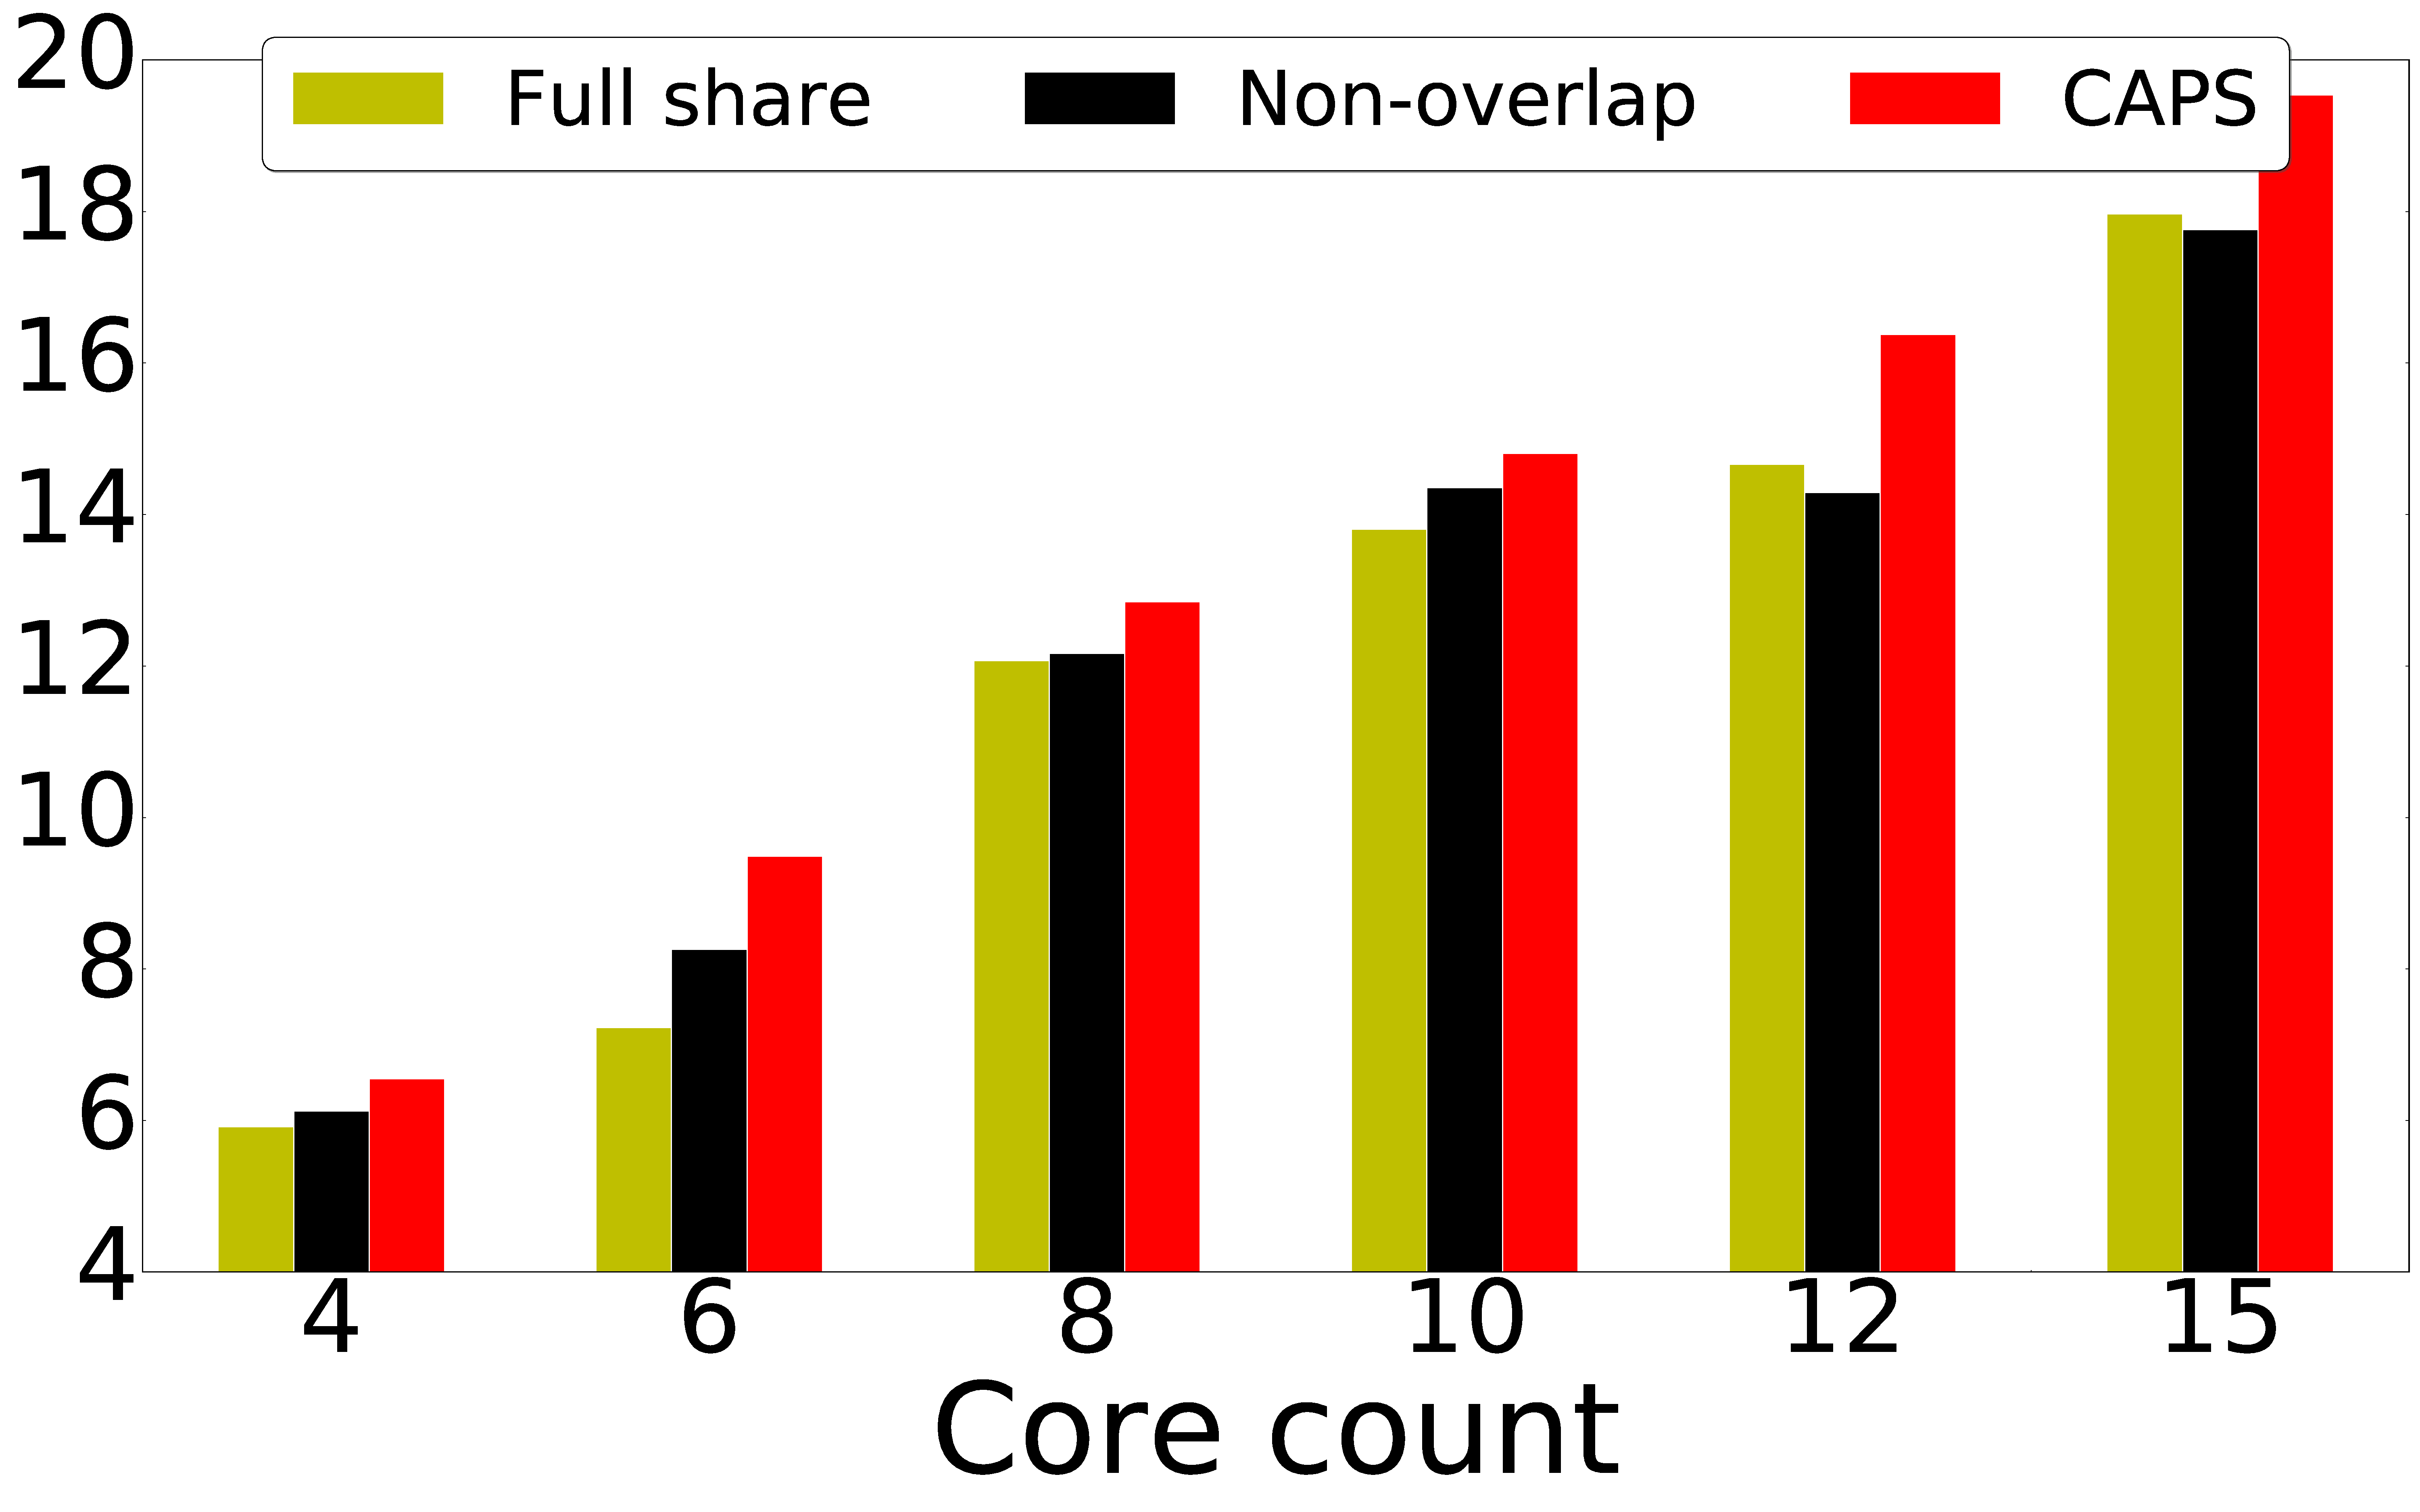
\includegraphics[width=0.9\linewidth]{figures/ipc.pdf}
        \caption{Throughput}
    \end{subfigure}
    \begin{subfigure}[b]{0.5\linewidth}
        \centering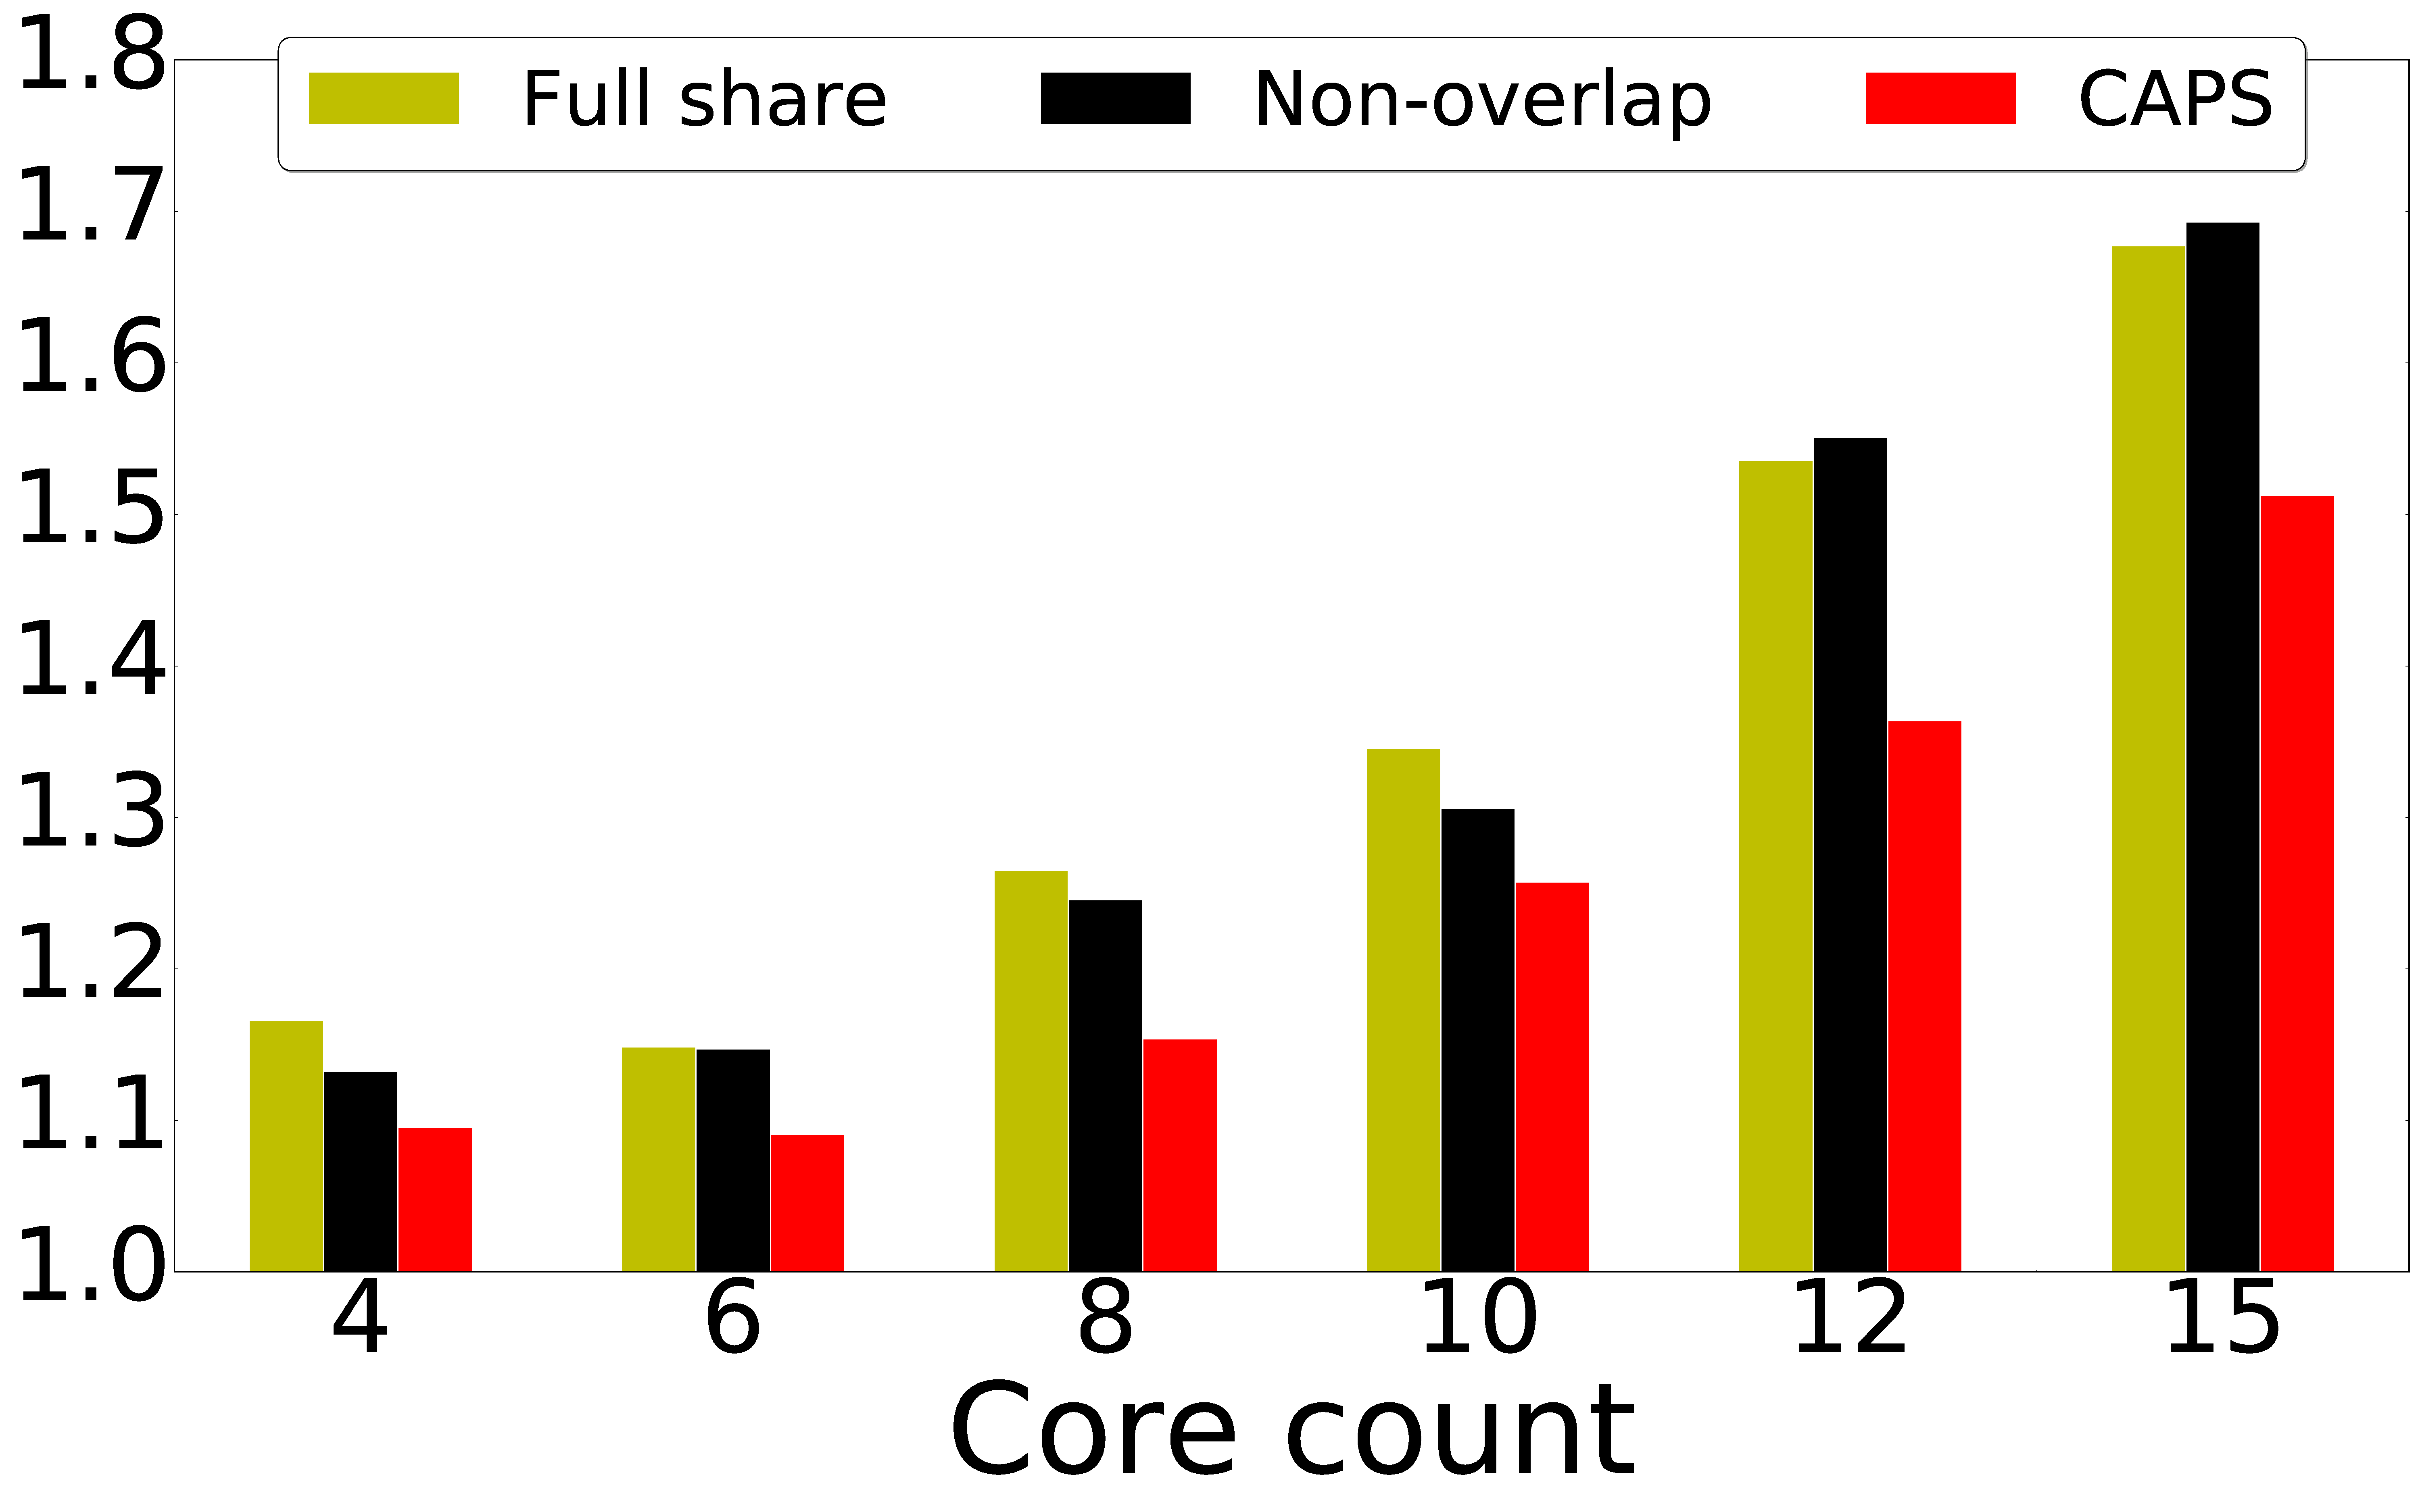
\includegraphics[width=0.9\linewidth]{figures/ws.pdf}
        \caption{Average slowdown}
    \end{subfigure}%
    \begin{subfigure}[b]{0.5\linewidth}
        \centering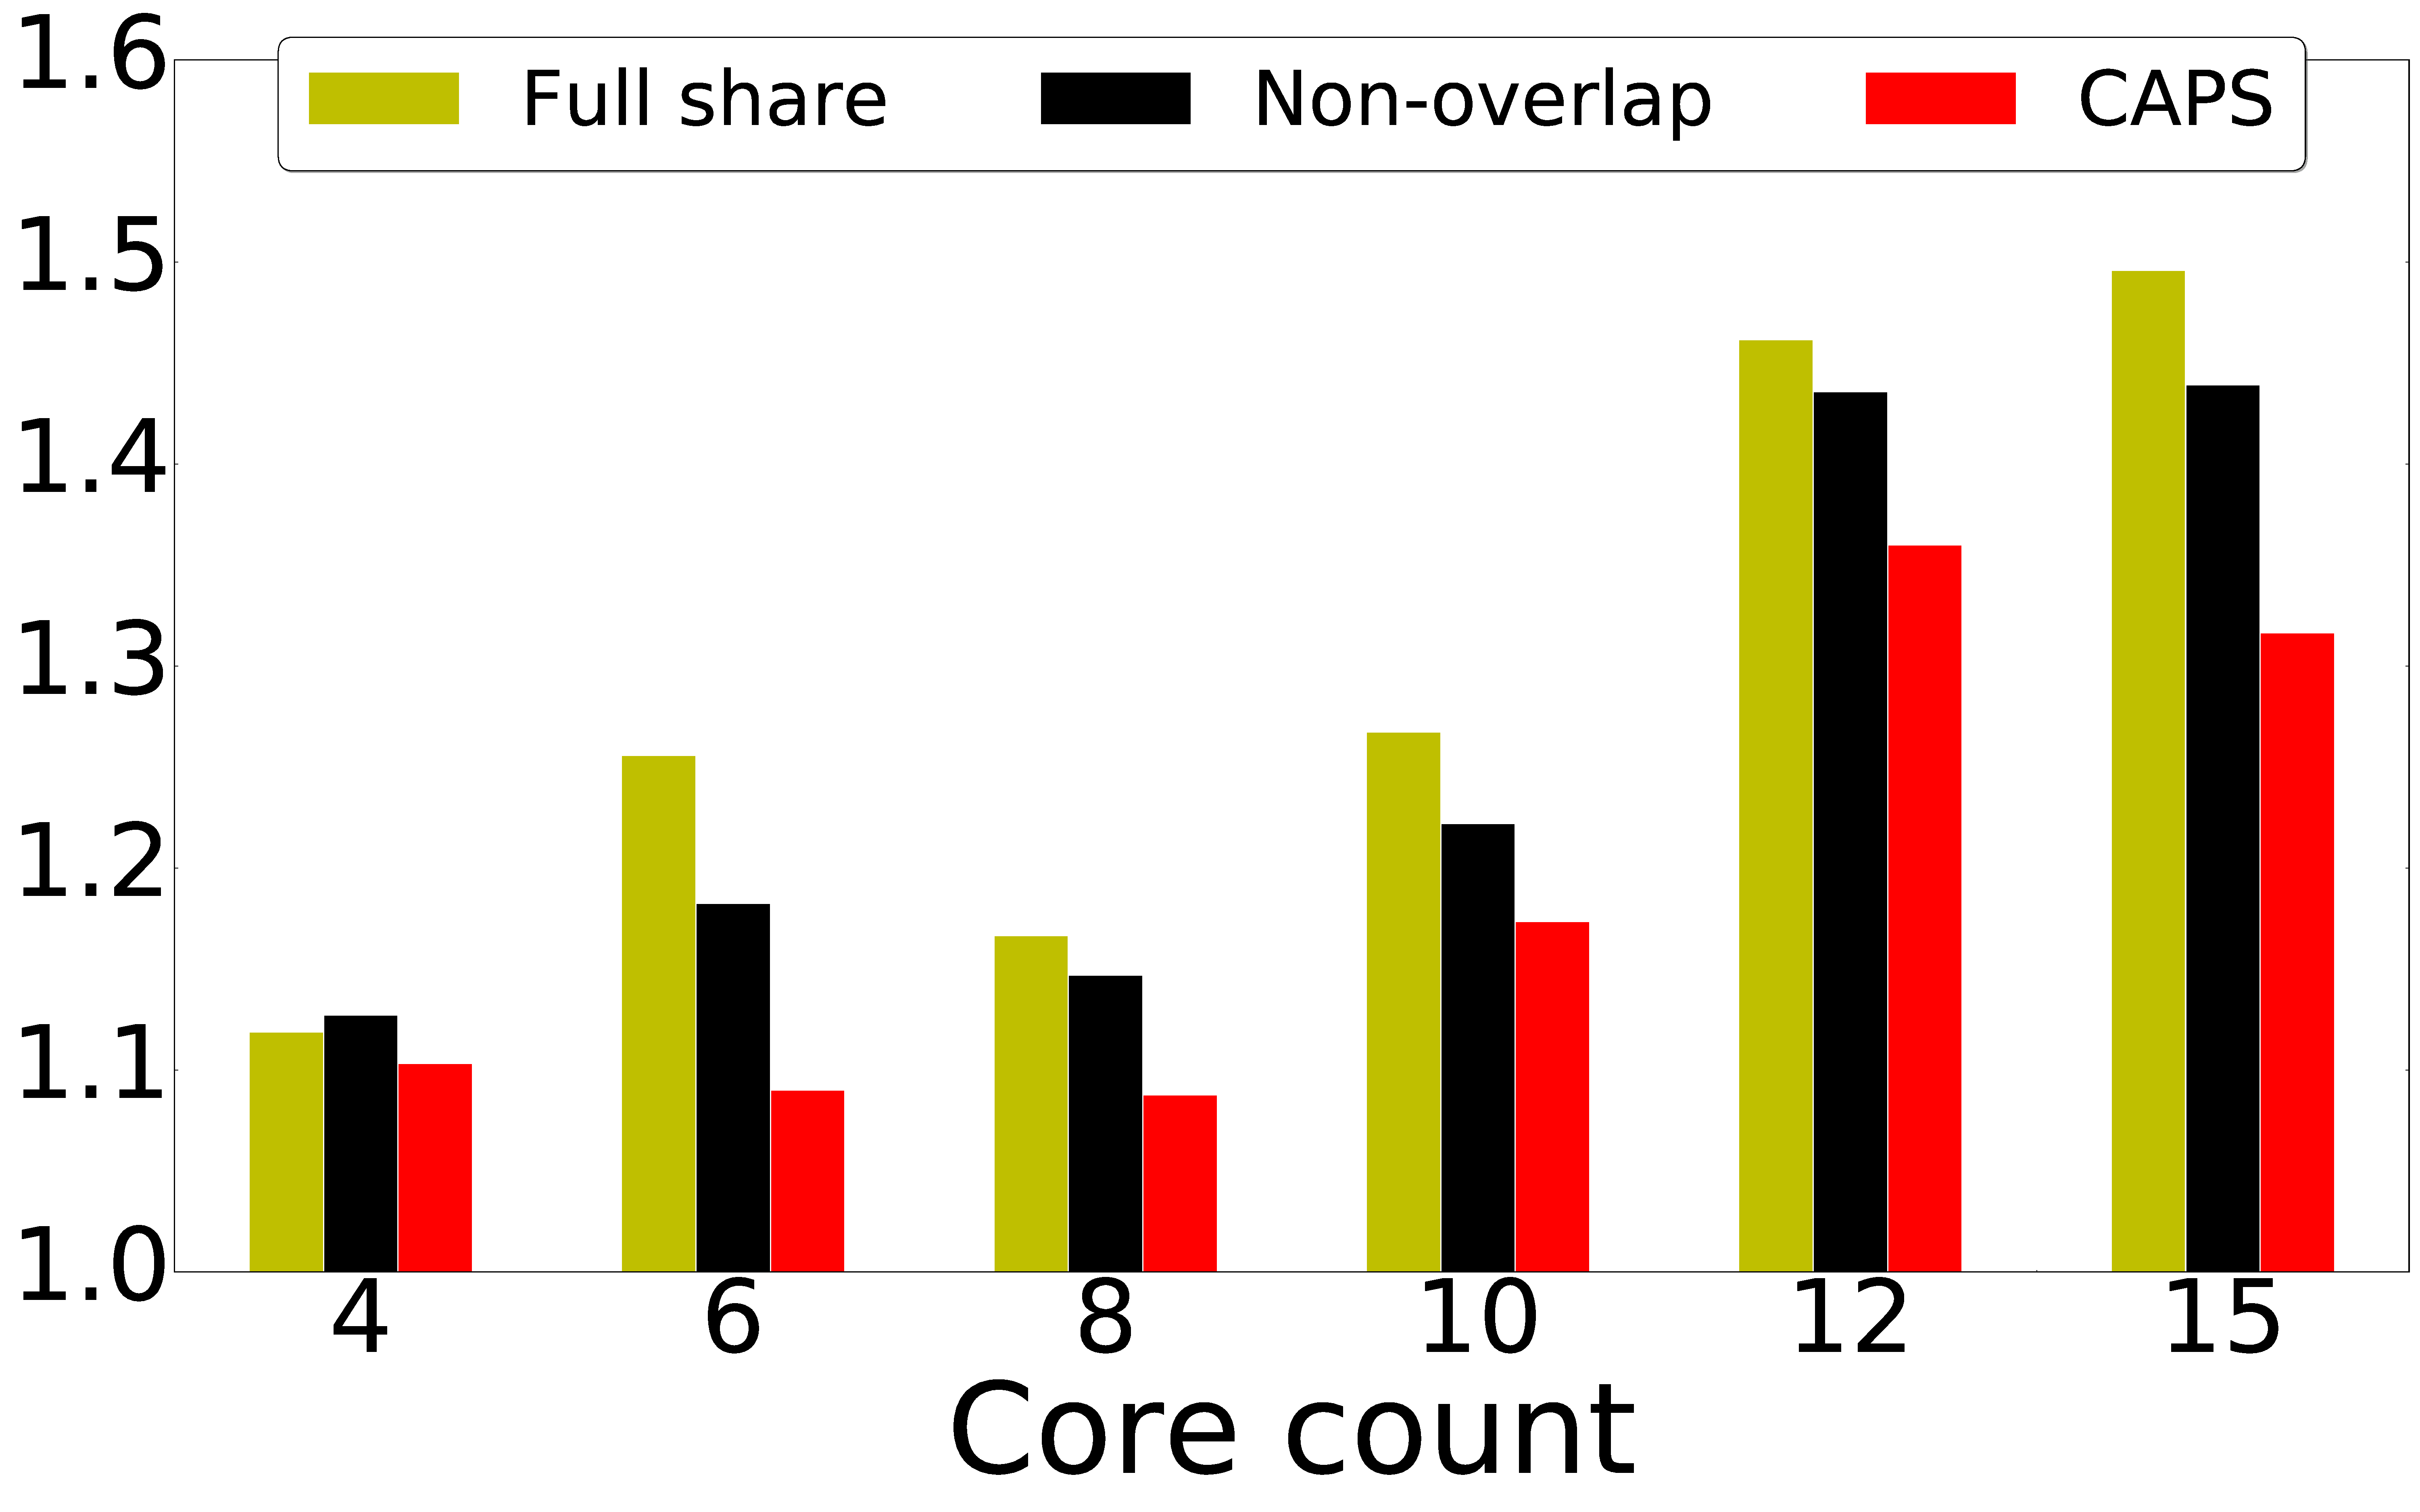
\includegraphics[width=0.9\linewidth]{figures/fs.pdf}
        \caption{Fair slowdown}
    \end{subfigure}
    \begin{subfigure}[b]{0.5\linewidth}
        \centering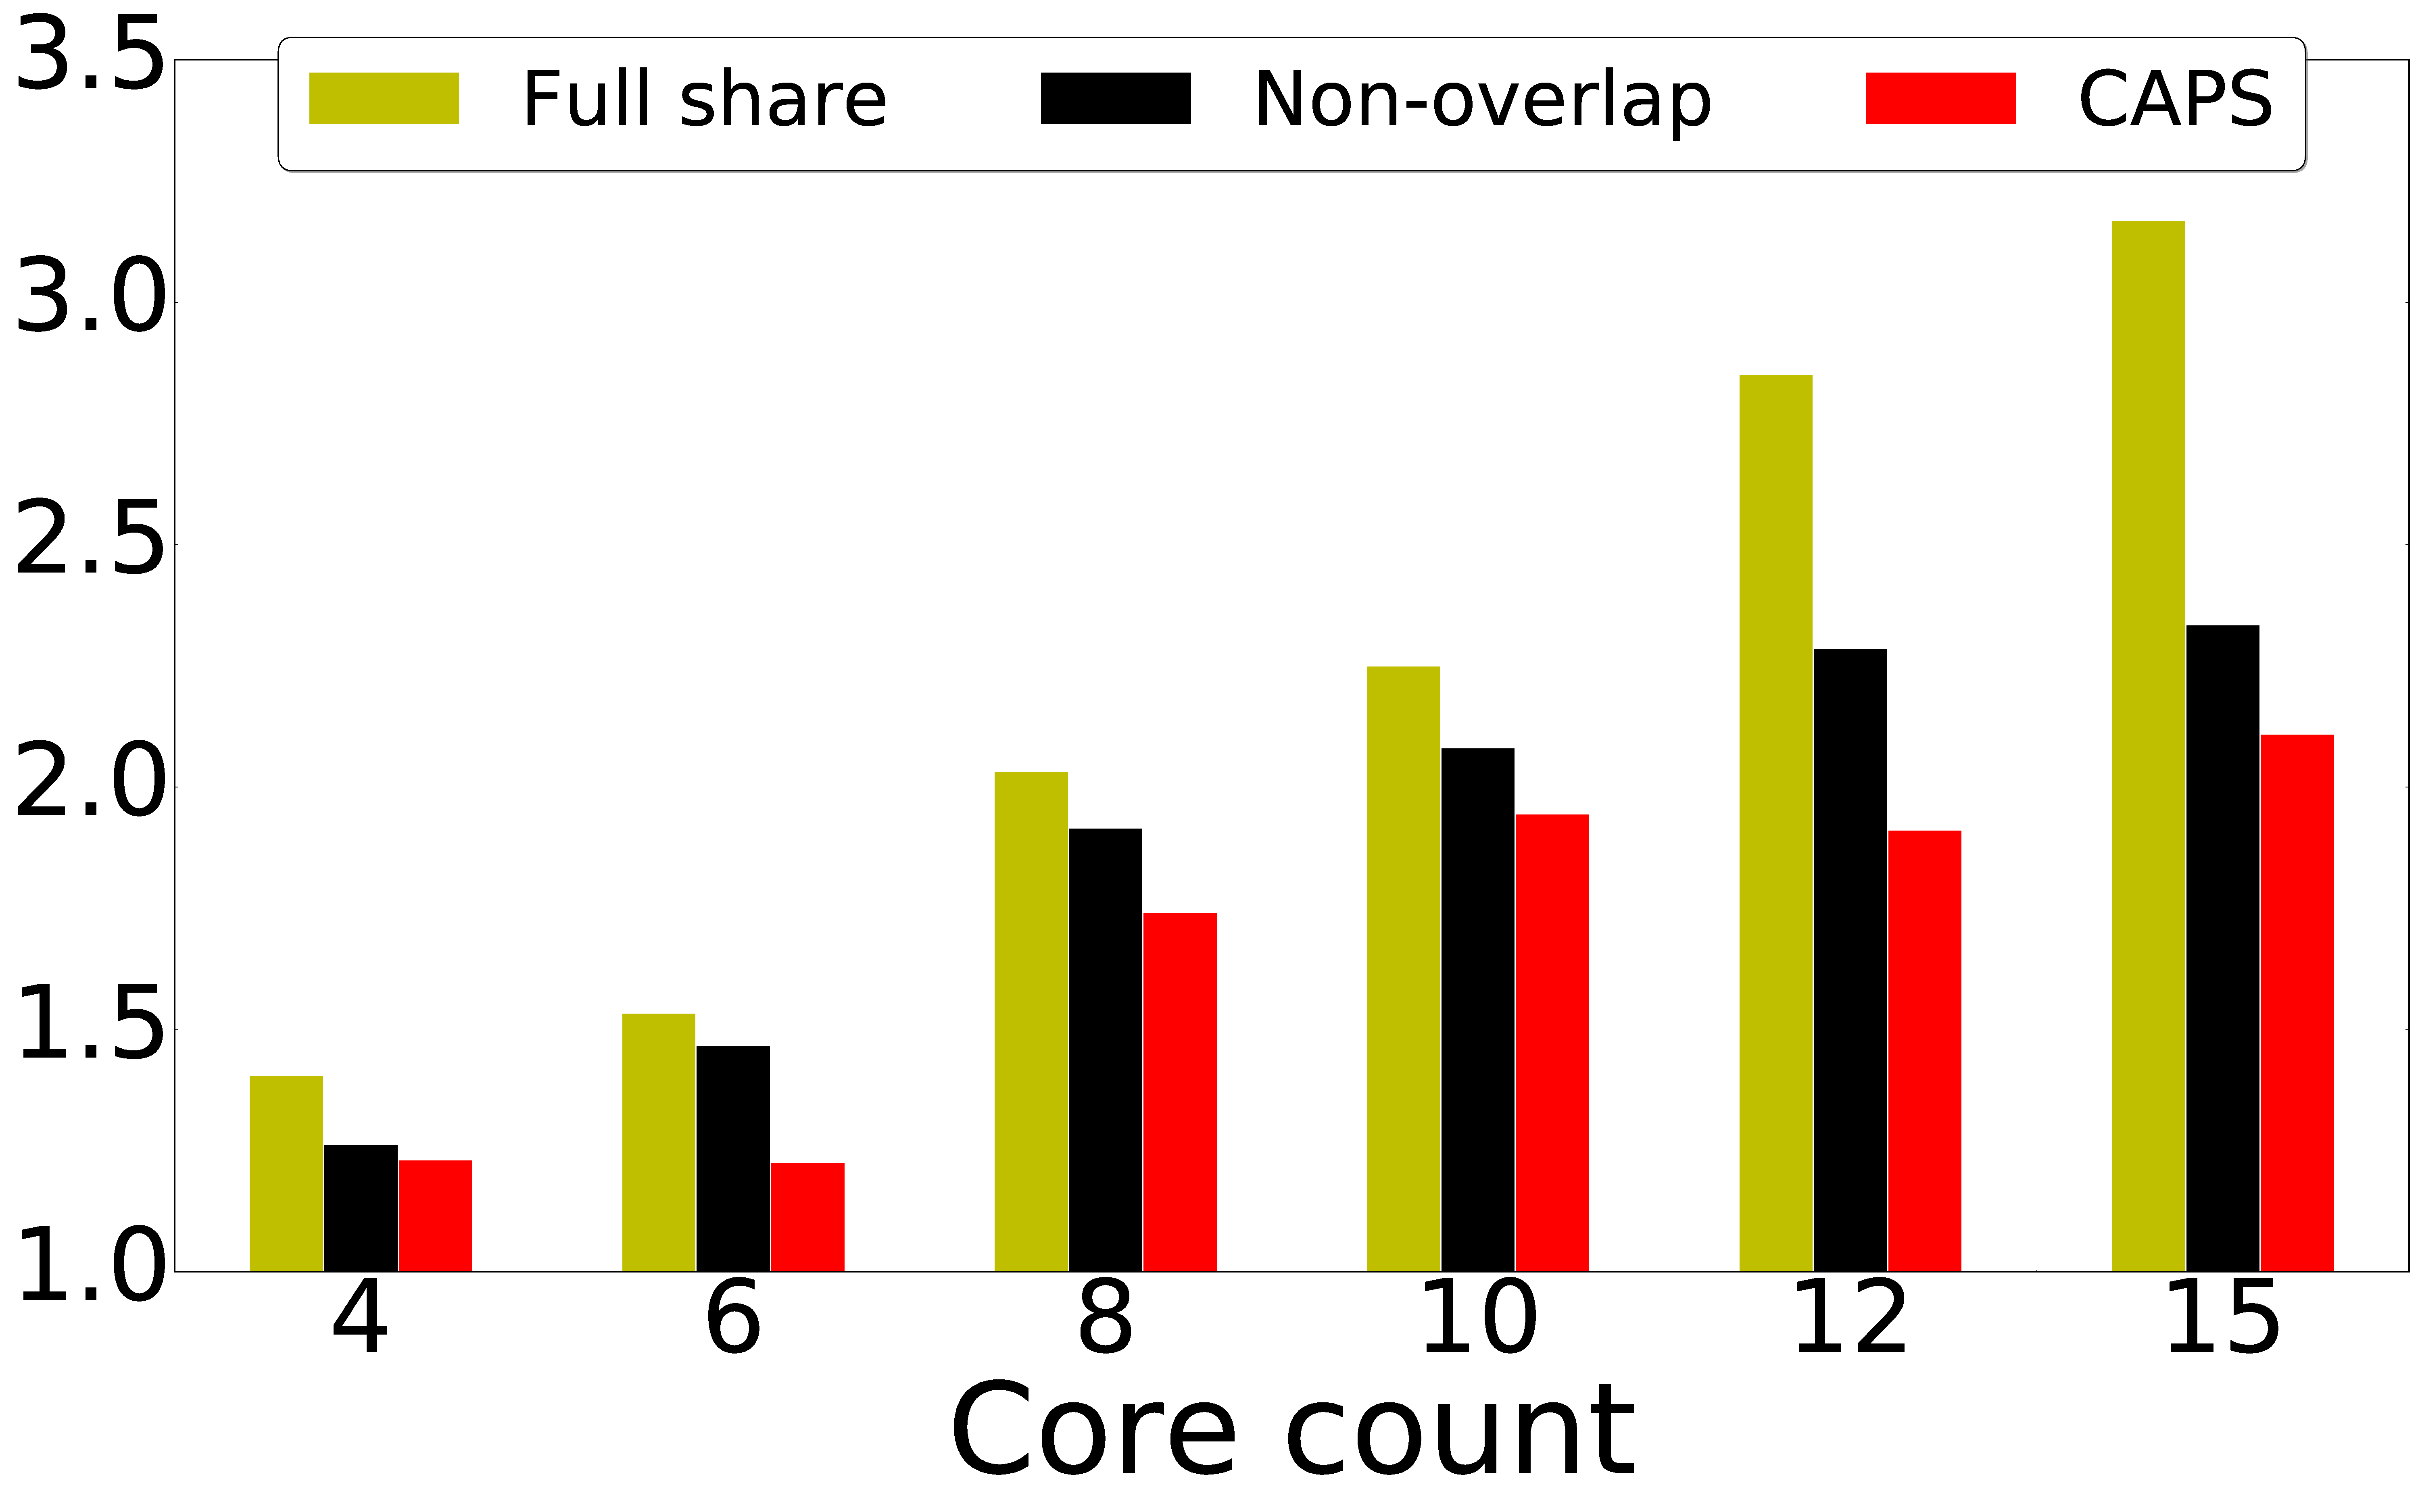
\includegraphics[width=0.9\linewidth]{figures/ms.pdf}
        \caption{Maximum slowdown}
    \end{subfigure}
    \caption{完全重叠、不重叠与CAPS部分重叠方案在不同核数下的5个优化指标对比}
    \label{fig:core_count}
\end{figure}

从图中可以看出,无论核数多少,CAPS生成的部分重叠方案基本上都是效果最好的方案。其次,随着核数的增加,对LLC的竞争愈发增加,性能下降也更为明显,这也给了CAPS更大的优化空间。可以看出随着核数的增加,CAPS对比自由竞争和不重叠的优势更加显著。特别地,在Average slowdown上,4核下CAPS平均可以把自由竞争下的1.166的Slowdown降低到1.095,优化效果达6.1\%,而在12核下,CAPS可以把1.536的Slowdown降低到1.364,提升效果达11.2\%。

不重叠分配方案在大多数情况下比自由竞争要稍微好一些。但是,随着核数的增加,不重叠方案的优化效果会越来差,在某些情况下甚至会起到反作用,比如在Average slowdown指标下12核和15核的情况,不重叠方案都比自由竞争还要差一点。之所以不重叠方案在高核数下效果不好,是因为其粒度过粗,不具有很好的扩展性。极端情况下当核数等于缓存路数的时候,该方案只能给每个核分配一个路,就彻底失去了灵活性,而只能起到隔离效果。与之不同的是,对于Maximum slowdown这个指标来说,不重叠方案相比于自由竞争方案能持续提供优化效果,这是因为该指标偏向于QoS,更加注重隔离干扰。在并发负载中,最严重Slowdown往往是由一个缓存非常敏感的程序引起的。不重叠的分配方案可以限制高污染性程序的缓存使用,使得敏感程序免受它们的干扰,这样Maximum slowdown就获得了优化。诚然如此,不重叠方案在各方面也是全面落后于CAPS部分重叠方案的。

可以观察到一个有趣的现象,在Fair slowdown下,8核相比6核的Slowdown反而更小了。这里的原因在于该指标注重公平性,因为不同的测试程序组合可能会对公平性造成不同的影响,新增的程序使得公平性更好或者更坏都有可能。  

\section{工作负载差异性的评估分析}

在本节中,我们对不同的工作负载组合进行评估分析。本评估重点针对10核的工作负载,通过不同的A类程序、B类程序和C类程序配比,每个负载包含10个各异的测试程序,一共产生25种组合。我们将这25个工作负载分别标记为“D1”到“D25”,配比详情如表\ref{tab:10w}所示。


\begin{table}[htbp]
\caption{10核工作负载配比表}
\label{tab:10w}
\centering
\begin{tabularx} {0.8\linewidth}{|X|l|l|l| } 
 \hline
 Label & TypeA & TypeB & TypeC \\
 \hline
D1 & 0 & 5 & 5 \\
\hline 
D2 & 2 & 2 & 6 \\
\hline 
D3, D4 & 2 & 5 & 3 \\
\hline 
D5, D6, D7 & 3 & 3 & 4 \\
\hline 
D8 & 3 & 4 & 3 \\
\hline 
D9, D10, D11 & 3 & 5 & 2 \\
\hline 
D12, D13, D14 & 4 & 3 & 3 \\
\hline 
D15, D16 & 5 & 0 & 5 \\
\hline 
D17 & 5 & 2 & 3 \\
\hline 
D18 & 5 & 3 & 2 \\
\hline 
D19 & 5 & 5 & 0 \\
\hline 
D20, D21, D22 & 6 & 2 & 2 \\
\hline 
D23 & 7 & 2 & 1 \\
\hline 
D24 & 8 & 1 & 1 \\
\hline 
D25 & 9 & 1 & 0 \\
\hline 
\end{tabularx}
\end{table}

\begin{figure}[htbp] 
    \centering
    \begin{subfigure}[b]{1\linewidth}
        \centering\includegraphics[width=0.95\linewidth]{figures/d20_miss.pdf}
        \caption{Average MPKI}
    \end{subfigure}
    \begin{subfigure}[b]{1\linewidth}
        \centering
\includegraphics[width=0.95\linewidth]{figures/d20_ipc.pdf}
        \caption{Throughput}
    \end{subfigure}
    \begin{subfigure}[b]{1\linewidth}
        \centering
\includegraphics[width=0.95\linewidth]{figures/d20_ws.pdf}
        \caption{Average slowdown}
    \end{subfigure}
    \begin{subfigure}[b]{1\linewidth}
        \centering
\includegraphics[width=0.95\linewidth]{figures/d20_fs.pdf}
        \caption{Fair slowdown}
    \end{subfigure}
    \begin{subfigure}[b]{1\linewidth}
        \centering\includegraphics[width=0.95\linewidth]{figures/d20_ms.pdf}
        \caption{Maximum slowdown}
    \end{subfigure}
    \caption{完全重叠、不重叠与CAPS部分重叠方案在10个并发负载下的5个优化指标对比}
    \label{fig:10w}
\end{figure}

实验结果如图\ref{fig:10w}所示。可以看到,CAPS基本上在每种工作负载的每种指标上都处于领先地位,除了D11的吞吐量。A类程序属于缓存敏感型,而B类属于不敏感且污染型, 当A类程序和B类程序在竞争使用LLC时,A类程序往往会因为B类程序的影响而导致严重的性能下降。所以当一个工作负载中A类和B类程序比较多时,自由竞争情况下的性能下降往往会比较严重,但在这种情况下CAPS往往能起到很好的优化效果。而在C类程序较多时,由于本身自由竞争下的性能损失也不大,所以留给CAPS的优化空间也较小。

同时,我们还观察到只要有一个污染性很大的程序就会对整个工作负载造成较大的影响。例如,D21和D18两个负载只差一个462.libquantum测试程序,D18把D21中的473.astar替换成462.libquantum,其余的程序都一样。然而,自由共享下的各项指标都变差了很多。462.libquantum是一个典型的B类程序,它的局部性较差,并不会从缓存占用中收益很多,但同时它的访存频率很高,在竞争情况下会占据大量空间,从而污染整个缓存空间。幸运的是,CAPS可以自动识别到这样的程序,然后限制它们的缓存使用,可以看到对于D18这组工作负载,CAPS都大大优化了5项指标的数值。

\section{个案分析}

在本节中,我们拿一个10核工作负载做更详细的分析。我们选择研究的负载是上节提到的D10,它是由10个程序组成:401.bzip2, 403.gcc, 429.mcf, 436.cactus, 465.tonto, 410.bwaves, 434.zeusmp, 437.leslie3d, 459.GemsFDTD和462.libquantum。这些程序中,前5个是A类敏感型程序,后5个是B类污染型程序。因为C类程序既不敏感也不污染,对整体的工作负载影响不大,考虑到典型性,所以本个案中就没有包含C类程序。图\ref{fig:case_scheme}展示了CAPS针对Throughput和Fair slowdown这两个优化指标所生成的方案。可以看到各个分配会有部分的重叠。光从分配方案上很难看出每个程序的实际占用是多少。因为一个看似很大的分配可能由于与多个程序竞争,实际占用的缓存空间会很小。为了更好的展示这两种分配方案的实际效果,我们使用缓存监控技术(CMT)实时测得了各个程序的实际缓存占用,这两种方案下以及自由竞争时各个程序的实际平均缓存占用如图\ref{fig:case_occu}所示。

\begin{figure}[htbp]
\centering
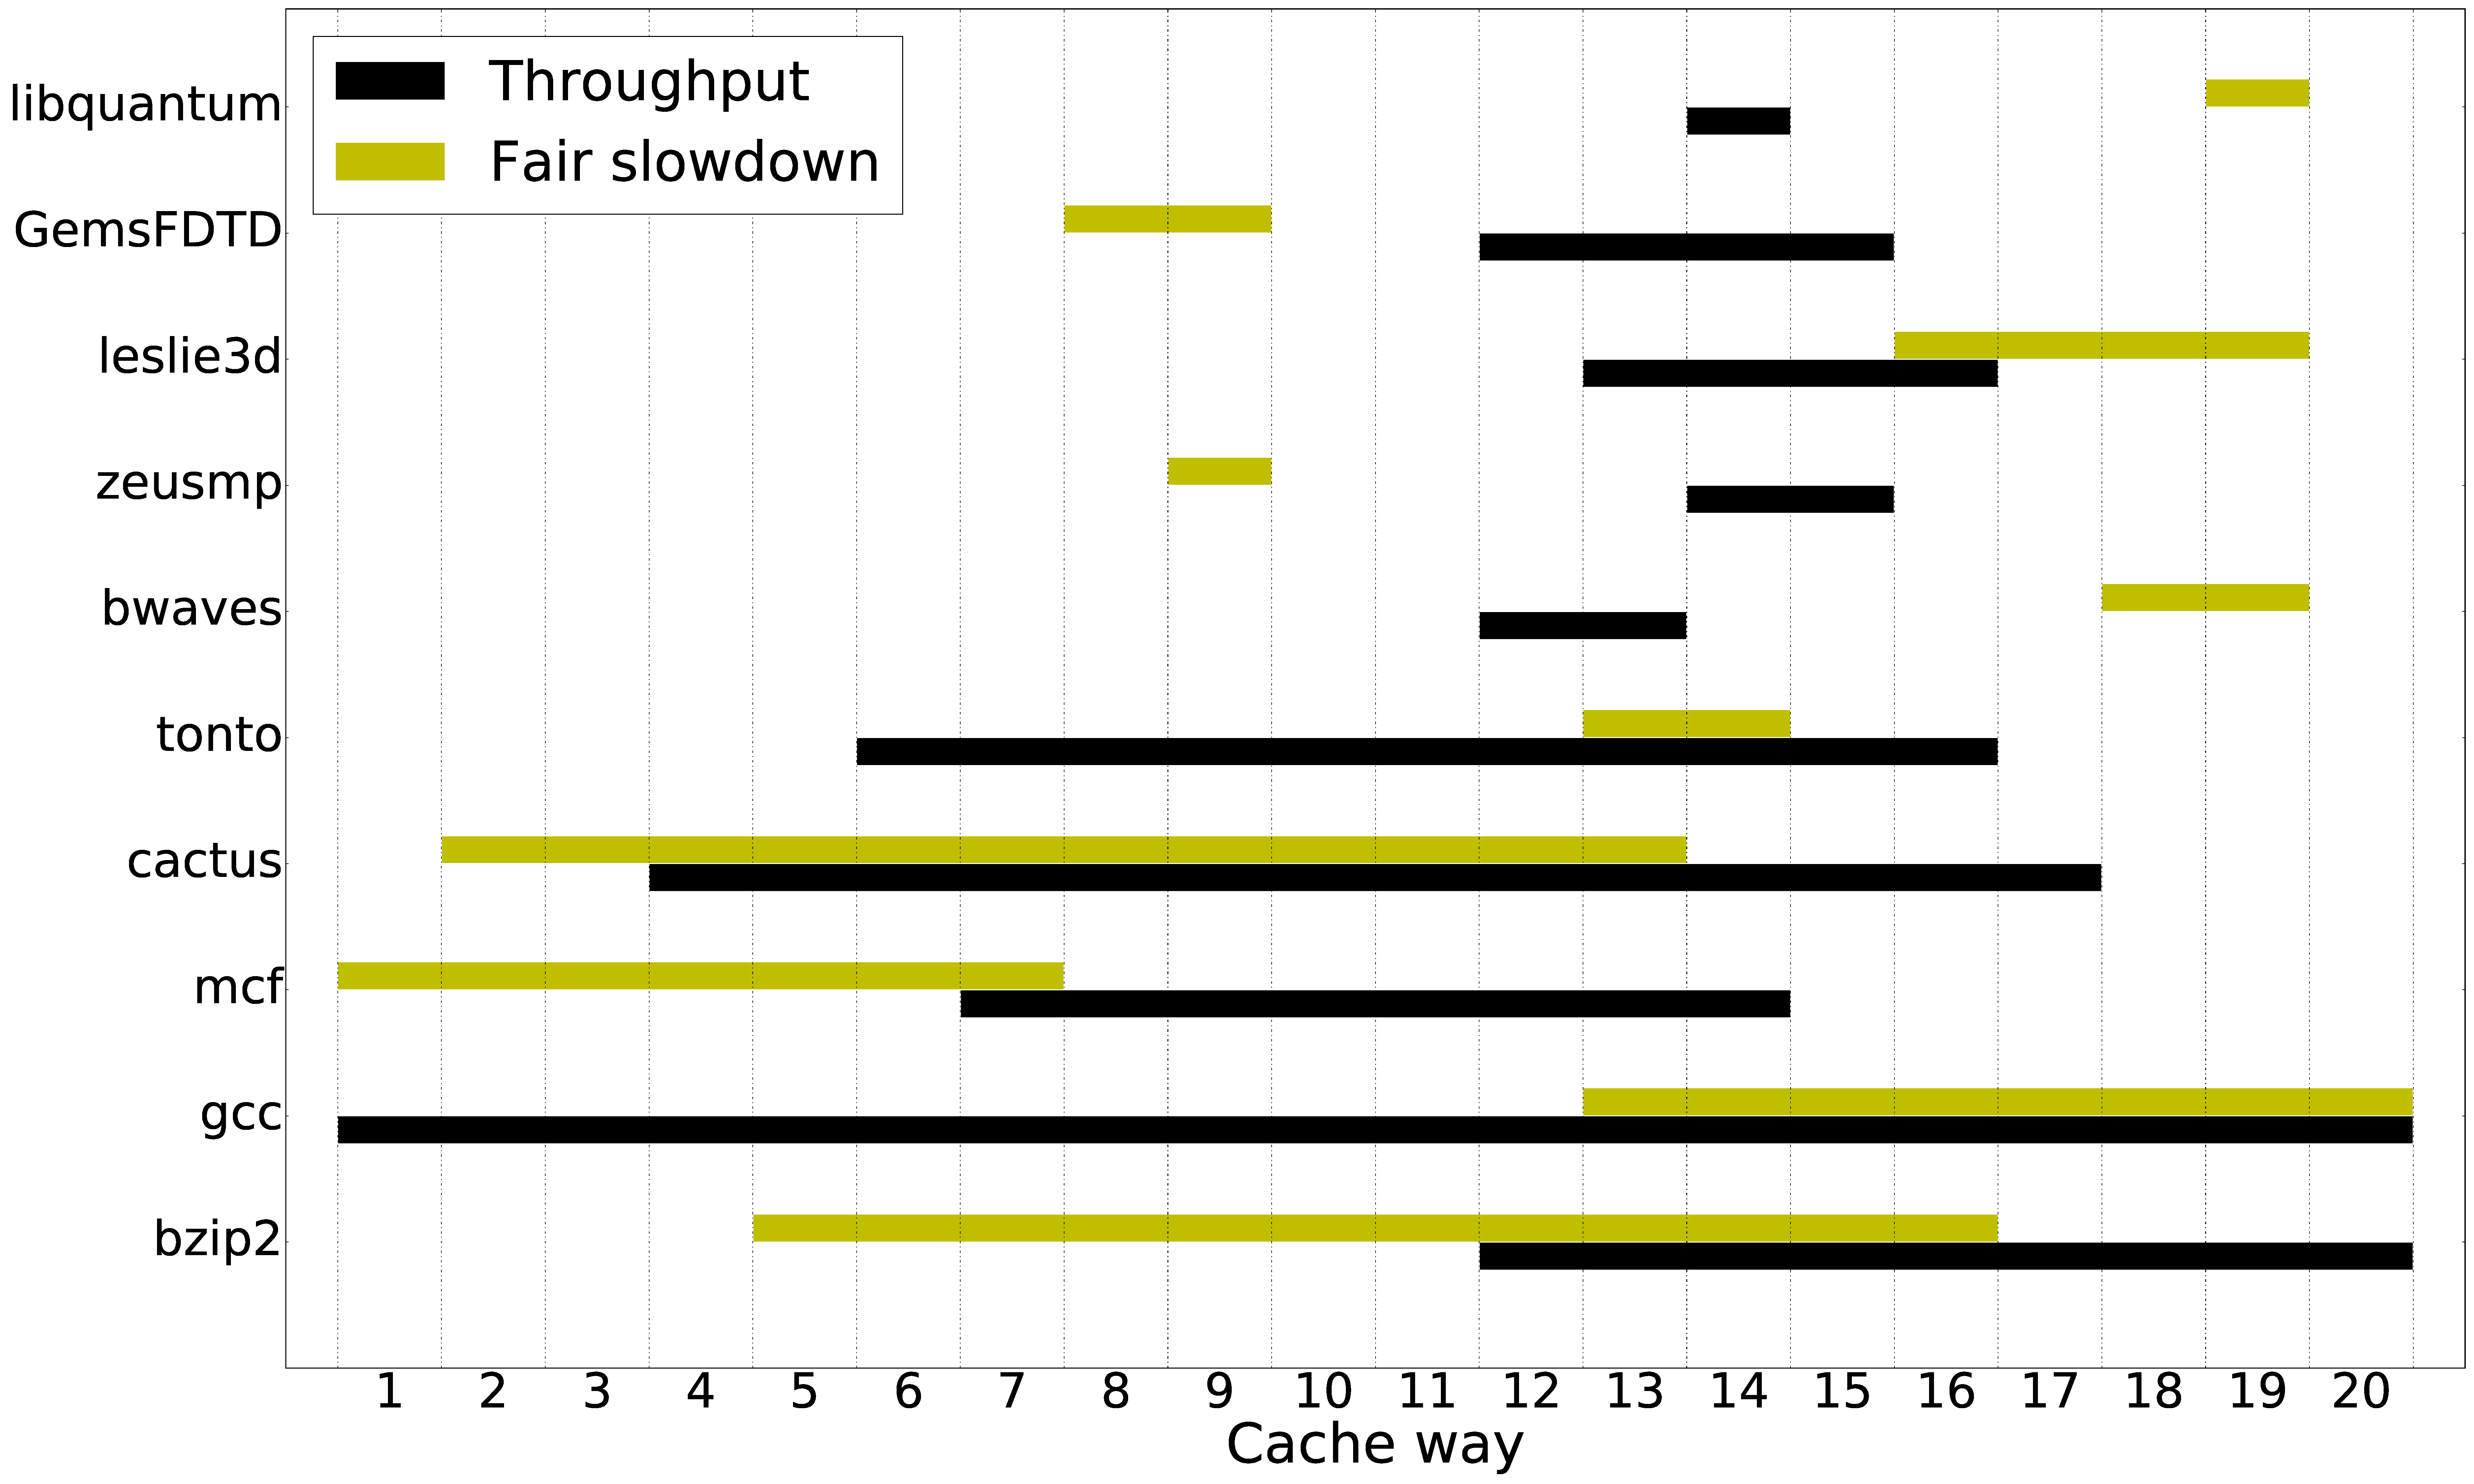
\includegraphics[width=0.95\columnwidth]{figures/case_study.pdf}
\caption{两种分别针对Throughput和Fair slowdown的CAPS分配方案}
\label{fig:case_scheme}
\end{figure} 

\begin{figure}[htbp]
\centering
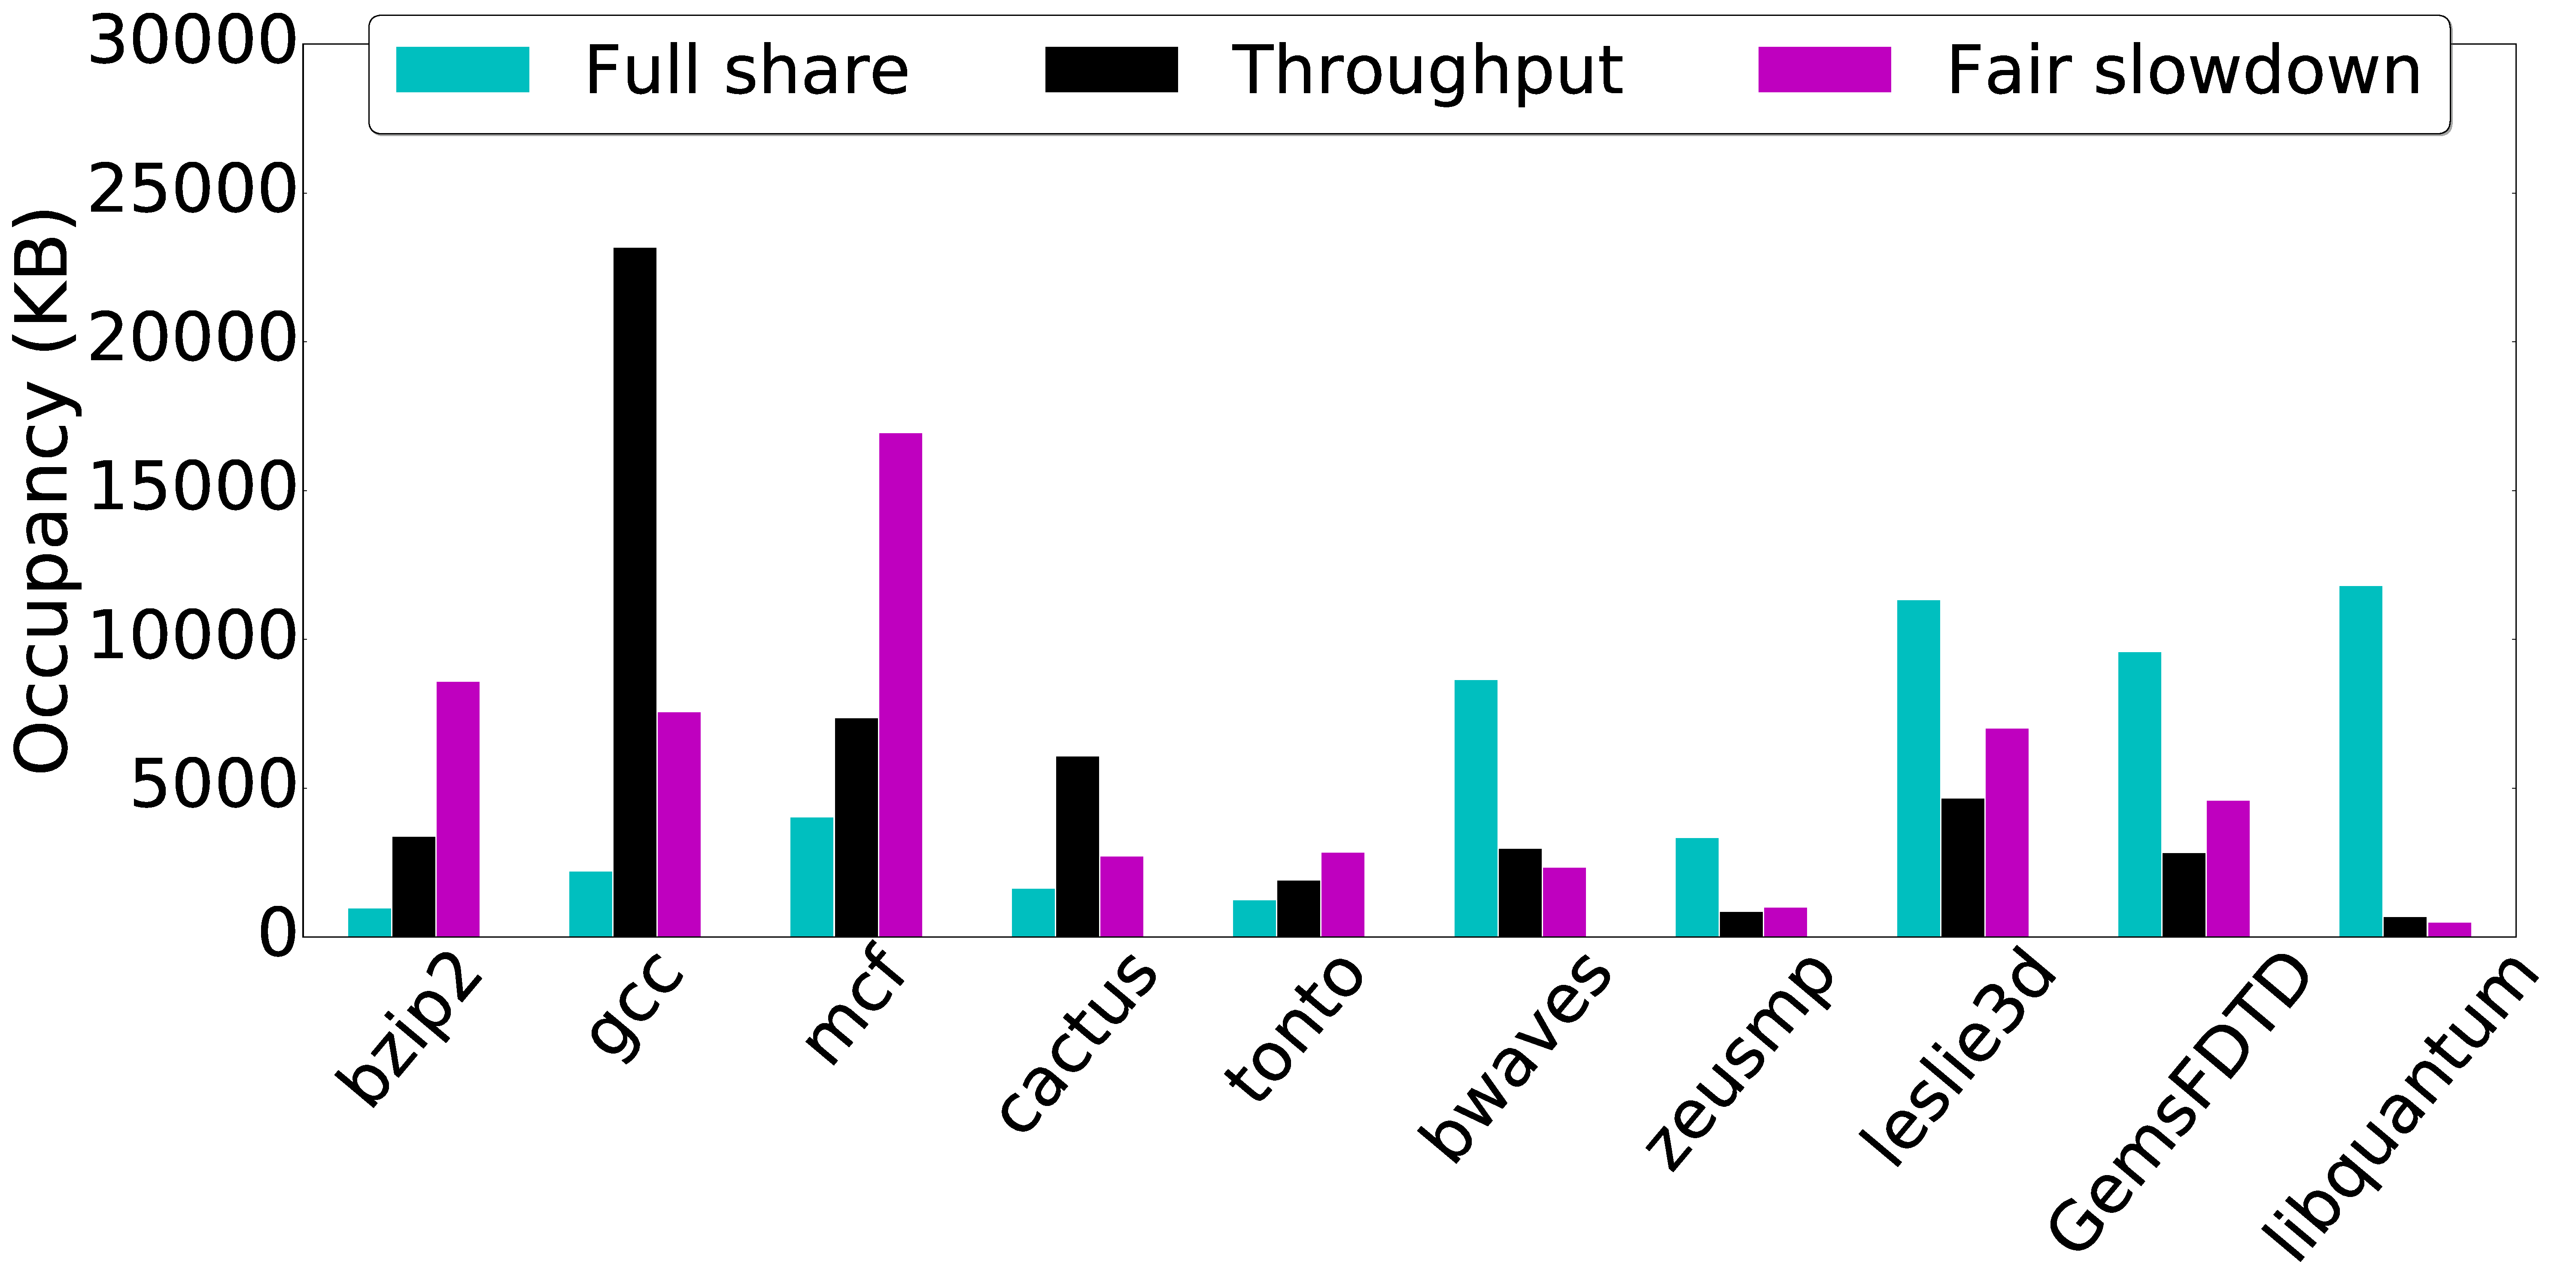
\includegraphics[width=0.9\linewidth]{figures/occ.pdf}
\caption{在自由竞争以及CAPS生成的Throughput和Fair slowdown方案下每个程序的实际缓存占用}
\label{fig:case_occu}
\end{figure} 

可以看出,无论是针对Throughput还是针对Fair slowdown的方案都为A类程序分配了较大的缓存空间,同时限制B类程序的缓存使用,这符合一般缓存优化的逻辑。正如所预料的,测试结果表明5个A类程序的IPC相比于完全竞争的情况都得到了显著的提高,同时B类程序虽然缓存空间被限制在较小的区域,但总体IPC变化幅度不大,所以工作负载总体性能指标就会获得提高,在图\ref{fig:case_ipc}中可以明显观察到这种趋势。然而,无论是针对何种目标的优化,CAPS都会自动地发现并限制B类污染性程序的缓存使用。


\begin{figure}[htbp]
\centering
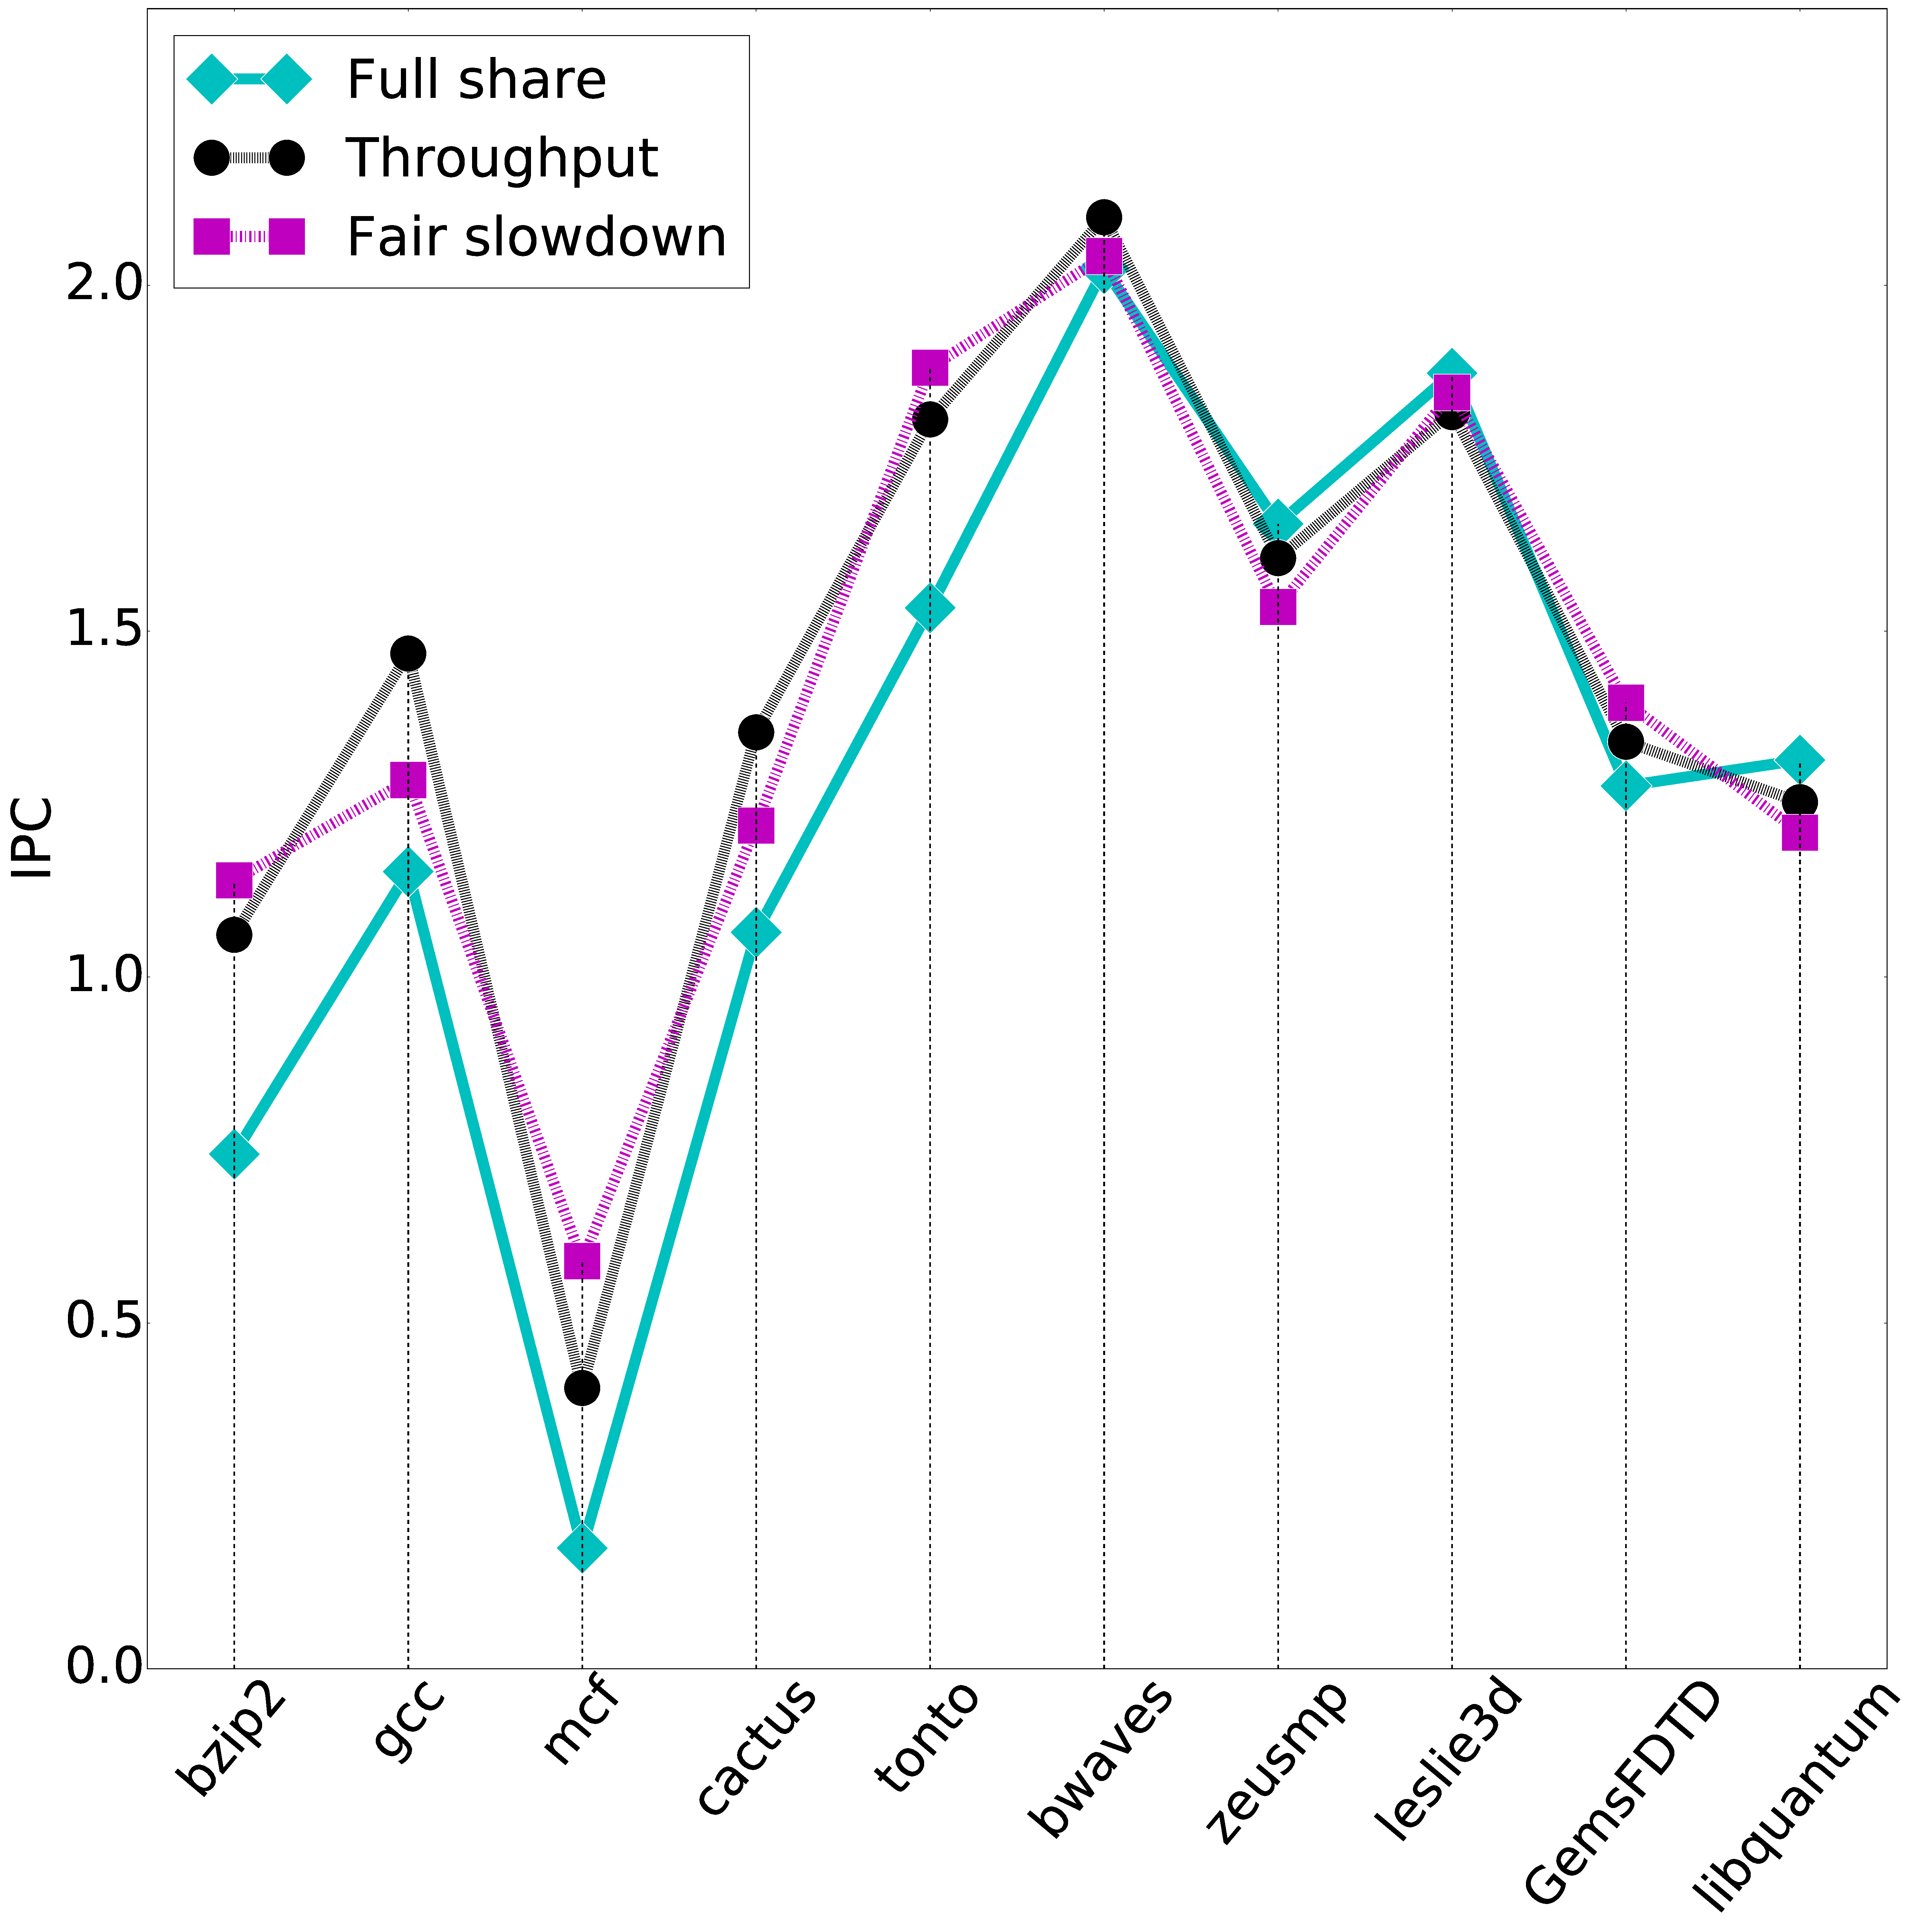
\includegraphics[width=0.8\columnwidth]{figures/case_ipc.pdf}
\caption{在自由竞争以及CAPS生成的Throughput和Fair slowdown方案下每个程序的IPC}
\label{fig:case_ipc}
\end{figure} 

虽然Throughput优化方案和Fair slowdown优化方案都会遵从多分配给A类程序、少分配给B类程序这一基本优化思路,但两种方案还是有一些不同之处。针对Throughput的吞吐量最大化方案会更加注重本身IPC就比较高的程序,因为提供同样大小的缓存给这类程序,往往在IPC数值的收益上会更大,而对于本身IPC较小的程序就会不太友好,因为从系统IPC的角度来看,给这类程序大量缓存空间并不会显著提高IPC的绝对数值。在另一方面,Fair slowdown策略关注的是IPC的变化率而不是绝对数值,因为slowdown就是通过IPC的变化比例来计算的,所以它对待高IPC和低IPC的程序会一视同仁。在这个D10的工作负载中,465.bzip2是一个高IPC程序,在单独运行的时候,它的IPC达到了1.70,而429.mcf是一个低IPC程序,它单独执行时的IPC只有0.58。在Throughput方案中,高IPC程序465.bzip相比于429.mcf得到了更大的缓存分配,因为这能大幅提升系统总体的IPC。而在Fair slowdown策略下,429.mcf的缓存分配反而比465.bzip更多,因为这能更好地缓解系统总体的slowdown。如图\ref{fig:case_ipc}所示,Throughput指标在Througput方案下是14.87,在Fair slowdown方案下是13.95;而Fair slowdown指在Throughput方案下是1.26,而在Fair slowdown方案下是1.21。与预期的一样,这两种方案都在各自锚定的指标上胜出了对方。